% ============================================================
%  INFORME TÉCNICO -- SEGUNDA ENTREGA
%  Álgebra Lineal Aplicada
%  Péndulo invertido sobre un carro (tres configuraciones)
%  Universidad Nacional de Colombia -- Sede Medellín
%  Mismo formato que el informe de la primera entrega.
% ============================================================
\documentclass[11pt,letterpaper]{article}

% ── Idioma y codificación ───────────────────────────────────
\usepackage[utf8]{inputenc}
\usepackage[T1]{fontenc}
\usepackage[spanish,provide=*]{babel}

% ── Tipografía ─────────────────────────────────────────────
\usepackage{mathpazo}
\usepackage{microtype}
\linespread{1.02}

% ── Geometría de página ─────────────────────────────────────
\usepackage[letterpaper,top=0.9in,bottom=0.9in,left=1in,right=1in]{geometry}

% ── Matemáticas ─────────────────────────────────────────────
\usepackage{amsmath,amssymb,amsthm,mathtools,bm}

% ── Color, cajas, tablas, figuras ───────────────────────────
\usepackage{xcolor}
\definecolor{acento}{RGB}{31,59,107}
\definecolor{acento2}{RGB}{120,40,40}
\usepackage[most]{tcolorbox}
\usepackage{booktabs}
\usepackage{array}
\usepackage{graphicx}
\usepackage{tikz}

% ── Títulos de sección ──────────────────────────────────────
\usepackage{titlesec}
\titleformat{\section}
  {\normalfont\large\bfseries\color{acento}}{\thesection}{0.7em}{}
\titleformat{\subsection}
  {\normalfont\normalsize\bfseries\color{acento!85!black}}{\thesubsection}{0.6em}{}
\titlespacing*{\section}{0pt}{1.1ex plus .8ex minus .2ex}{0.6ex plus .2ex}
\titlespacing*{\subsection}{0pt}{0.9ex plus .6ex minus .2ex}{0.45ex plus .2ex}

% ── Encabezado/pie ──────────────────────────────────────────
\usepackage{fancyhdr}
\pagestyle{fancy}\fancyhf{}
\renewcommand{\headrulewidth}{0.4pt}
\fancyhead[L]{\footnotesize\itshape Informe técnico (segunda entrega) --- Péndulo invertido}
\fancyhead[R]{\footnotesize\itshape Álgebra Lineal Aplicada}
\fancyfoot[C]{\thepage}

% ── Listas y enlaces ────────────────────────────────────────
\usepackage{enumitem}
\setlist{itemsep=1.5pt,topsep=2pt}
\usepackage[colorlinks=true,linkcolor=acento,citecolor=acento2,urlcolor=acento]{hyperref}
\usepackage{cleveref}

% ── Código ──────────────────────────────────────────────────
\usepackage{listings}
\definecolor{codecmt}{RGB}{110,120,130}
\definecolor{codekw}{RGB}{31,59,107}
\definecolor{codestr}{RGB}{120,40,40}
\lstdefinestyle{julia}{%
  basicstyle=\ttfamily\scriptsize,
  keywordstyle=\color{codekw}\bfseries,
  commentstyle=\color{codecmt}\itshape,
  stringstyle=\color{codestr},
  showstringspaces=false,
  breaklines=true,
  columns=fullflexible,
  frame=single,
  rulecolor=\color{acento!45!black},
  framesep=4pt,
  xleftmargin=6pt,xrightmargin=6pt,
  aboveskip=6pt,belowskip=6pt,
  morekeywords={function,end,for,while,if,else,elseif,return,using,import,module,struct,begin,in}
}
\lstset{style=julia}

% ── Rutas de figuras ────────────────────────────────────────
% Las figuras propias de este informe se generan en figs/; los cuatro mapas
% del atlas los produce ../atlas/make_atlas_figs.jl y se toman de ahí para no
% duplicar ni el cálculo ni los archivos.
\graphicspath{{figs/}{../atlas/figs/}}

% ── Teoremas ────────────────────────────────────────────────
\theoremstyle{definition}
\newtheorem{definicion}{Definición}[section]
\newtheorem{ejemplo}[definicion]{Ejemplo}
\theoremstyle{plain}
\newtheorem{teorema}[definicion]{Teorema}
\newtheorem{proposicion}[definicion]{Proposición}
\newtheorem{lema}[definicion]{Lema}
\newtheorem{corolario}[definicion]{Corolario}
\theoremstyle{remark}
\newtheorem{observacion}[definicion]{Observación}
\renewcommand{\qedsymbol}{$\blacksquare$}

% ── Cajas ───────────────────────────────────────────────────
\newtcolorbox{clave}[1][]{colback=acento!4,colframe=acento!55!black,
  boxrule=0.6pt,arc=2pt,left=6pt,right=6pt,top=5pt,bottom=5pt,#1}
\newtcolorbox{alerta}[1][]{colback=acento2!4,colframe=acento2!60!black,
  boxrule=0.6pt,arc=2pt,left=6pt,right=6pt,top=5pt,bottom=5pt,#1}

% ── Operadores ──────────────────────────────────────────────
\DeclareMathOperator{\rank}{rango}
\DeclareMathOperator{\Imo}{Im}
\DeclareMathOperator{\gen}{gen}
\DeclareMathOperator{\Real}{Re}
\DeclareMathOperator{\diag}{diag}
% El espectro se denota con la sigma matematica. NO usar \DeclareMathOperator
% aqui: pondria \sigma en modo texto y con la codificacion T1 se imprime "oe".
\newcommand{\spec}{\sigma}
\newcommand{\R}{\mathbb{R}}
\newcommand{\C}{\mathbb{C}}
\newcommand{\calC}{\mathcal{C}}
\newcommand{\calO}{\mathcal{O}}
\newcommand{\calE}{\mathcal{E}}
\newcommand{\xv}{\bm{x}}
\newcommand{\uv}{\bm{u}}
\newcommand{\yv}{\bm{y}}
\newcommand{\ev}{\bm{e}}
\newcommand{\rv}{\bm{r}}
\newcommand{\Mm}{\bm{M}}
\newcommand{\Gm}{\bm{G}}
\newcommand{\Fm}{\bm{F}}

% ── cleveref en español ─────────────────────────────────────
\crefname{equation}{ec.}{ecs.}\Crefname{equation}{Ecuación}{Ecuaciones}
\crefname{section}{sección}{secciones}\Crefname{section}{Sección}{Secciones}
\crefname{figure}{figura}{figuras}\Crefname{figure}{Figura}{Figuras}
\crefname{table}{tabla}{tablas}\Crefname{table}{Tabla}{Tablas}
\crefname{definicion}{definición}{definiciones}\Crefname{definicion}{Definición}{Definiciones}
\crefname{teorema}{teorema}{teoremas}\Crefname{teorema}{Teorema}{Teoremas}
\crefname{proposicion}{proposición}{proposiciones}\Crefname{proposicion}{Proposición}{Proposiciones}
\crefname{observacion}{observación}{observaciones}\Crefname{observacion}{Observación}{Observaciones}
\crefname{appendix}{apéndice}{apéndices}\Crefname{appendix}{Apéndice}{Apéndices}
\AtBeginDocument{%
  \renewcommand{\crefpairconjunction}{ y }%
  \renewcommand{\creflastconjunction}{ y }%
  \renewcommand{\crefmiddleconjunction}{, }%
}
\addto\captionsspanish{\renewcommand{\tablename}{Tabla}}

% ============================================================
\begin{document}

% ── Portada ─────────────────────────────────────────────────
\begin{center}
    {\footnotesize\bfseries\color{acento2} INFORME TÉCNICO --- SEGUNDA ENTREGA}\\[0.4em]
    {\LARGE\bfseries Cuándo el Álgebra Lineal Deja de Bastar \\[0.2em]
     y qué la Reemplaza}\\[0.5em]
    {\large Péndulo Triple, Márgenes de Controlabilidad, \\ Fronteras de Operabilidad y Estimación de Estado}\\[1.2em]
    {\normalsize Mateo Bedoya Rojas \quad\textbullet\quad Camilo Alejandro Patiño Osorio \quad\textbullet\quad Santiago Uribe Echavarría}\\[0.5em]
    {\footnotesize
    Facultad de Ciencias, Universidad Nacional de Colombia, Sede Medellín \\ \texttt{mabedoyar@unal.edu.co} \quad \texttt{cpatinoo@unal.edu.co} \quad \texttt{sauribee@unal.edu.co}}\\[0.8em]
\end{center}
\vspace{0.4em}
\hrule height 0.6pt
\vspace{1.0em}

% ── Resumen ─────────────────────────────────────────────────
\begin{abstract}
\noindent
La primera entrega estableció que el péndulo invertido, en sus configuraciones
simple y doble, es inestable pero controlable y observable, y lo estabilizó con
realimentación de estado. Esta segunda entrega ataca los cinco huecos que
quedaban. Primero se sustituyen las dos deducciones separadas por una
\emph{familia genérica de $N$ eslabones}, de la que las configuraciones I y II
son casos particulares y en la que la Configuración III ---el péndulo triple,
con estado en $\R^8$--- es el siguiente término. Segundo, se muestra
experimentalmente que el criterio de rango de Kalman, siendo un teorema
correcto, es un mal algoritmo: el condicionamiento de $\calC$ crece unos cuatro
órdenes de magnitud por eslabón y con cinco alcanza $1/\varepsilon_{\text{máq}}$.
Se lo sustituye por el \emph{margen de Popov--Belevitch--Hautus}, que por el
teorema de Eckart--Young mide la distancia en norma 2 a la incontrolabilidad y
decae suavemente. Tercero, se construye un \emph{atlas de operabilidad} que
barre el espacio de parámetros y separa la imposibilidad estructural de la
práctica, delimitando dónde el controlador sirve y dónde no. Cuarto, se cierra
el argumento de observabilidad con un \emph{observador de Luenberger} diseñado
por dualidad de Kalman, cuyo principio de separación se demuestra en dos líneas
de álgebra lineal. Quinto, todo queda blindado por 618 pruebas de regresión que
contrastan los jacobianos analíticos contra diferenciación automática y
reproducen cada cifra publicada. Varias predicciones del plan de trabajo
resultaron incorrectas al medirlas; se documentan explícitamente.
\end{abstract}

\vspace{0.3em}
\noindent\textbf{Palabras clave:}\;
péndulo triple, test PBH, distancia a la incontrolabilidad, valores singulares,
Eckart--Young, condicionamiento, elipsoide invariante, dualidad de Kalman,
principio de separación, exponencial matricial, retenedor de orden cero.
\vspace{0.8em}
\hrule height 0.4pt
\vspace{1.0em}

% ============================================================
\section{Qué añade esta entrega}
\label{sec:problema}

La primera entrega~\cite{entrega1} recorrió, para dos configuraciones, la cadena
completa
\[
\begin{gathered}
\text{Euler--Lagrange} \to \Mm(q)\ddot q=\text{rhs} \to \text{linealización} \to (A,B,C)\\
\to \spec(A),\ \rank\calC,\ \rank\calO \to K \to \text{simulación}.
\end{gathered}
\]
El resultado fue sólido, pero un lector crítico podía señalar cinco huecos. Esta
entrega los ataca uno por uno.

\begin{enumerate}
  \item \textbf{La observabilidad se analizaba y no se usaba.} Se demostraba
  $\rank\calO=n$ y acto seguido se controlaba con $\uv=-K\xv$, es decir con el
  estado \emph{completo}, que en un sistema real no se mide. Se resuelve en la
  \cref{sec:observador}.

  \item \textbf{No había noción de límite de validez.} Se reportaba que el LQR
  estabiliza desde $\theta_0=0.40$~rad, pero no hasta dónde llega ni con qué
  actuador. Se resuelve en la \cref{sec:atlas}.

  \item \textbf{El criterio de rango es frágil y no se decía.} $\rank\calC$ es
  una decisión binaria tomada con una tolerancia numérica implícita. Se resuelve
  en las \cref{sec:condicionamiento,sec:pbh}.

  \item \textbf{No había pruebas automatizadas.} Los jacobianos analíticos
  estaban escritos a mano y nada comprobaba su corrección de forma
  reproducible. Se resuelve en la \cref{sec:metodologia}.

  \item \textbf{Solo dos puntos en el eje de complejidad.} Con dos casos, la
  afirmación ``el mismo razonamiento escala'' es anecdótica; con tres se vuelve
  una curva. Se resuelve en las \cref{sec:generico,sec:configiii}.
\end{enumerate}

\begin{clave}
\small
\textbf{La tesis de esta entrega.} El álgebra lineal que resuelve el problema
escala sin cambios conceptuales al crecer el número de eslabones, pero
\emph{el condicionamiento no}. Llega un punto en que los teoremas siguen siendo
ciertos y los algoritmos que los implementan dejan de ser confiables. La
respuesta no es cambiar de teoría sino de herramienta: sustituir criterios
binarios de rango por medidas continuas basadas en valores singulares.
\end{clave}

% ============================================================
\section{Formalización genérica en $N$ eslabones}
\label{sec:generico}

En vez de deducir una tercera configuración desde cero, se reformula el problema
para $N$ eslabones arbitrarios. Esto tiene una consecuencia práctica de primer
orden: el modelo genérico puede \emph{validarse} contra los dos ya entregados, de
modo que su corrección no se pide por fe sino que se demuestra numéricamente.

\subsection{Coordenadas y convenciones}

Se consideran $N$ eslabones articulados en serie sobre un carro. Las coordenadas
generalizadas son
\[
q=(x,\ \theta_1,\ \dots,\ \theta_N)\in\R^{N+1},
\]
con $x$ la posición horizontal del carro y $\theta_j$ el ángulo del eslabón $j$
medido desde la \emph{vertical superior}. Los ángulos son \emph{absolutos}
respecto a la vertical, no relativos al eslabón anterior: es la convención de la
primera entrega y se conserva. El espacio de estados es el fibrado tangente
$T\mathcal{Q}\cong\R^{2(N+1)}$, con el orden intercalado del proyecto
\[
\xv=(x,\ \dot x,\ \theta_1,\ \omega_1,\ \dots,\ \theta_N,\ \omega_N)^{\!\top}.
\]
La entrada sigue siendo escalar, $u\in\R$: \textbf{$N+1$ grados de libertad y un
solo actuador}. La subactuación pasa de $2\!:\!1$ en la Configuración~I a
$3\!:\!1$ en la II y a $4\!:\!1$ en la III.

Cada eslabón se describe con cuatro parámetros: masa $m_j$, longitud $\ell_j$,
distancia $a_j$ de la articulación inferior al centro de masa, y momento de
inercia $I_j$ respecto a ese centro. La distinción entre $\ell_j$ y $a_j$ es la
que permite unificar los dos modelos previos: $\ell_j$ determina dónde se
articula el eslabón siguiente, y $a_j$ determina el momento estático. Para una
barra uniforme $a_j=\ell_j/2$ e $I_j=\tfrac{1}{12}m_j\ell_j^2$; para una masa
puntual en el extremo, $a_j=\ell_j$ e $I_j=0$.

\subsection{Las tres agrupaciones que organizan el modelo}

Al expandir las energías cinética y potencial aparecen tres agrupaciones de
parámetros que estructuran todo el desarrollo. Para $j=1,\dots,N$:
\begin{equation}
\boxed{\ \beta_j=m_ja_j+\ell_j\!\!\sum_{i>j}m_i\ },\qquad
\boxed{\ J_j=I_j+m_ja_j^2+\ell_j^2\!\!\sum_{i>j}m_i\ },\qquad
\boxed{\ \Gamma_{jk}=\ell_{\min(j,k)}\,\beta_{\max(j,k)}\ }
\label{eq:agrupaciones}
\end{equation}

Su lectura física es directa. El momento estático $\beta_j$ recoge la masa
propia del eslabón por su brazo más la longitud completa del eslabón por la masa
de todo lo que carga encima. La inercia efectiva $J_j$ es el momento de inercia
respecto a \emph{su} articulación, con el término de Steiner y la carga de los
superiores. El acoplamiento $\Gamma_{jk}$ mide cuánto se acelera el eslabón $j$
cuando se acelera el $k$.

Con estas definiciones la energía potencial se escribe de forma notablemente
compacta:
\begin{equation}
V=g\sum_{j=1}^{N}\beta_j\cos\theta_j.
\label{eq:potencial}
\end{equation}

\begin{observacion}[Por qué inestabilidad y controlabilidad están ligadas]
\label{obs:beta}
El mismo $\beta_j$ que acopla el carro con el eslabón $j$ en la energía
\emph{cinética} es el que pesa la gravedad sobre ese eslabón en la
\emph{potencial} \cref{eq:potencial}. La coincidencia no es casual: ambos
provienen del mismo momento estático. Es la razón estructural de que la
inestabilidad y la controlabilidad estén ligadas en este sistema: \emph{el canal
por el que la gravedad desestabiliza es el mismo por el que el carro puede
actuar}. Si $\beta_j$ fuera cero, el eslabón $j$ ni caería ni podría
controlarse.
\end{observacion}

\subsection{Ecuaciones de movimiento}

Aplicando $\frac{d}{dt}\frac{\partial L}{\partial\dot q_i}-\frac{\partial L}{\partial q_i}=Q_i$
con $L=T-V$ se obtiene, para el carro,
\begin{equation}
\Big(M+\sum_i m_i\Big)\ddot x+\sum_{j}\beta_j\big(\cos\theta_j\,\ddot\theta_j-\sin\theta_j\,\dot\theta_j^2\big)+b\,\dot x=u,
\label{eq:eomcarro}
\end{equation}
y para el eslabón $j$,
\begin{equation}
\beta_j\cos\theta_j\,\ddot x+J_j\ddot\theta_j+\sum_{k\neq j}\Gamma_{jk}\big[\cos(\theta_j-\theta_k)\,\ddot\theta_k+\sin(\theta_j-\theta_k)\,\dot\theta_k^2\big]=g\beta_j\sin\theta_j.
\label{eq:eomeslabon}
\end{equation}

En forma mecánica estándar $\Mm(q)\ddot q+C(q,\dot q)\dot q+G(q)=\Fm u$, la
matriz de masa es
\begin{equation}
\Mm(q)=\begin{pmatrix}
M+\sum_i m_i & \beta_1\cos\theta_1 & \cdots & \beta_N\cos\theta_N\\
\beta_1\cos\theta_1 & J_1 & \cdots & \Gamma_{1N}\cos(\theta_1-\theta_N)\\
\vdots & \vdots & \ddots & \vdots\\
\beta_N\cos\theta_N & \Gamma_{N1}\cos(\theta_N-\theta_1) & \cdots & J_N
\end{pmatrix},
\label{eq:massmatrix}
\end{equation}
simétrica y definida positiva por ser la Hessiana de $T$ respecto a $\dot q$.
Esto justifica resolver $\Mm(q)\ddot q=\text{rhs}$ por factorización de Cholesky
en lugar de una LU genérica o, peor, invirtiendo la matriz.

El \textbf{signo positivo} de $g\beta_j\sin\theta_j$ en el lado derecho de
\cref{eq:eomeslabon} es la firma de la inestabilidad: para $\theta_j$ pequeño el
término vale $+g\beta_j\theta_j$, una realimentación positiva. Es el mismo
mecanismo que el $+(M+m)mgL/D_0$ de la Configuración~I.

\subsection{Las configuraciones I y II como casos particulares}
\label{sec:casosparticulares}

Instanciando \cref{eq:agrupaciones}:

\textbf{$N=1$, barra uniforme} (con la notación de la Configuración~I, en la que
$L$ es la distancia al centro de masa y por tanto $\ell_1=2L$ es la longitud
completa de la barra: $a_1=\ell_1/2=L$ e $I_1=\tfrac{1}{12}m\ell_1^2=\tfrac{1}{12}m(2L)^2$,
sin eslabones superiores): $\beta_1=mL$ y $J_1=I+mL^2$. La ecuación del carro queda
$(M+m)\ddot x+mL(\cos\theta\,\ddot\theta-\sin\theta\,\dot\theta^2)+b\dot x=u$ y
la del péndulo $mL\cos\theta\,\ddot x+(I+mL^2)\ddot\theta=mgL\sin\theta$. Es
exactamente el modelo de la Configuración~I, línea por línea.

\textbf{$N=2$, masas puntuales} ($a_j=\ell_j$, $I_j=0$):
\[
\beta_1=(m_1+m_2)L_1,\quad \beta_2=m_2L_2,\quad
J_1=(m_1+m_2)L_1^2,\quad J_2=m_2L_2^2,\quad \Gamma_{12}=m_2L_1L_2,
\]
que reproduce término a término la matriz de masa y el lado derecho de la
Configuración~II, \emph{incluidos los signos de los términos centrífugos}.

\begin{clave}
\small
\textbf{Esto es una prueba, no una afirmación.} Los modelos de las
Configuraciones I y II se conservan intactos y coexisten con el genérico. La
comparación entre ambos es por tanto un contraste entre \emph{dos
implementaciones independientes de la misma física}. Medida sobre 20 estados
aleatorios por configuración, la discrepancia máxima es de $5.3\times10^{-15}$
para $N=1$ y \emph{exactamente cero} para $N=2$: no solo coinciden dentro de
tolerancia, sino que producen las mismas operaciones de punto flotante en el
mismo orden. Un refactor destructivo habría eliminado esta prueba.
\end{clave}

% ============================================================
\section{Configuración III: el péndulo triple}
\label{sec:configiii}

\subsection{Parámetros y por qué estos}

Los parámetros por defecto se eligen para que la comparación con la
Configuración~II sea \emph{limpia}: la misma masa total de péndulo (0.6~kg) y la
misma longitud total (1~m), redistribuidas en tres barras uniformes en lugar de
dos masas puntuales. Así, cualquier diferencia observada es atribuible a la
estructura y no a un cambio de escala.

\begin{table}[htbp]
  \centering\small
  \caption{Parámetros por defecto de la Configuración III.}
  \label{tab:paramsiii}
  \begin{tabular}{@{}llc@{}}
    \toprule
    \textbf{Parámetro} & \textbf{Valor} & \textbf{Justificación}\\
    \midrule
    $M$ & 1.0 kg & igual que I y II\\
    $m_1=m_2=m_3$ & 0.2 kg & total 0.6 kg, igual que la Config.~II\\
    $\ell_1=\ell_2=\ell_3$ & $1/3$ m & total 1 m, igual que I y II\\
    $a_j$ & $\ell_j/2=1/6$ m & barra uniforme\\
    $I_j$ & $\tfrac{1}{12}m_j\ell_j^2=1.852\times10^{-3}$ kg\,m$^2$ & barra uniforme\\
    $g$ & 9.81 m/s$^2$ & igual que I y II\\
    $b$ & 0.1 N\,s/m & igual que la Config.~I\\
    \bottomrule
  \end{tabular}
\end{table}

Con ellos, $\beta=(0.16667,\ 0.1,\ 0.03333)$ y
$J=(0.05185,\ 0.02963,\ 0.00741)$.

\subsection{Linealización y predicción estructural del espectro}
\label{sec:linealizacion}

Evaluando en $\theta_j=0$, $\dot q=0$, $u=0$ se tiene $\cos\to1$,
$\sin\theta_j\to\theta_j$, $\cos(\theta_j-\theta_k)\to1$, y los términos
cuadráticos en las velocidades desaparecen por ser de segundo orden. Lo que
queda es un sistema lineal con \emph{matriz de masa constante}:
\begin{equation}
\Mm_0\,\ddot q=\Gm_0\,q-\Fm_0\,\dot q+\bm{e}_1u,
\label{eq:linealizado}
\end{equation}
con $\Mm_0=\Mm(0)$, $\Gm_0=g\diag(0,\beta_1,\dots,\beta_N)$ y $\Fm_0$ la matriz
de fricción. Despejando se obtienen los tres bloques
\[
A_{cc}=\Mm_0^{-1}\Gm_0,\qquad A_{cv}=-\Mm_0^{-1}\Fm_0,\qquad
B_c=\Mm_0^{-1}\bm{e}_1,
\]
que se ensamblan directamente en el orden intercalado. En orden por bloques la
matriz sería $\begin{psmallmatrix}0&I\\A_{cc}&A_{cv}\end{psmallmatrix}$, que es
esta misma conjugada por una permutación: el espectro no cambia, pero se
ensambla la versión intercalada por coherencia con las otras configuraciones.

\begin{proposicion}[Estructura del espectro sin fricción]
\label{prop:espectro}
Si $\Fm_0=0$, los eigenvalores de $A$ vienen en pares $\pm\lambda$ más un cero
doble:
\[
\spec(A)=\{\pm\lambda_1,\dots,\pm\lambda_N,\ 0,\ 0\},
\]
de modo que hay exactamente $N$ modos inestables.
\end{proposicion}

\begin{proof}
Buscando soluciones de la forma $q(t)=v\,e^{\lambda t}$ en
\cref{eq:linealizado} con $\Fm_0=0$ y $u=0$ se obtiene el problema generalizado
de eigenvalores $\Gm_0 v=\lambda^2\Mm_0 v$. Por tanto los eigenvalores de $A$
son las \emph{raíces cuadradas} de los de $\Mm_0^{-1}\Gm_0$, y aparecen en pares
$\pm\lambda$. Como $\Gm_0$ tiene una fila y una columna nulas ---el carro no
tiene fuerza recuperadora---, $\Mm_0^{-1}\Gm_0$ es singular y contribuye
$\lambda=0$ con multiplicidad dos, en un bloque de Jordan
$2\times2$~\cite{hoffman1971,olver2018}.
\end{proof}

Esta proposición es una \emph{predicción a priori}, no un ajuste a posteriori:
se verifica computacionalmente para $N=1,\dots,5$ antes de mirar ningún número
concreto. La fricción del carro rompe ligeramente la simetría y desdobla el
cero: en la Configuración~III con $b=0.1$ se obtiene $\{0,\,-0.0625\}$ en lugar
de $\{0,0\}$.

\subsection{Resultados de lazo abierto}

El espectro obtenido es
\begin{equation}
\spec(A)=\{+18.0613,\ +9.7740,\ +4.3777,\ 0,\ -0.0625,\ -4.3990,\ -9.7813,\ -18.0647\},
\label{eq:espectroiii}
\end{equation}
con \textbf{tres modos inestables} y la estructura casi antisimétrica predicha
por la \cref{prop:espectro}. El modo dominante $\lambda_{\max}=18.06$~s$^{-1}$
implica una constante de tiempo de caída de $1/\lambda_{\max}=55$~ms: el sistema
se desploma \emph{cuatro veces más rápido} que la Configuración~I.

Los rangos de Kalman son plenos: $\rank\calC=\rank\calO=8$. Con
$Q=\diag(1,0,10,0,10,0,10,0)$ y $R=0.1$ ---los mismos pesos de las otras dos
configuraciones, extendidos--- el LQR da
\[
K=(-3.16,\ -6.17,\ -317.43,\ -4.37,\ 911.95,\ 37.73,\ -667.37,\ -61.42),
\qquad \|K\|_2=1176.0,
\]
\[
\spec(A-BK)=\{-0.84\pm0.79i,\ -4.57\pm2.32i,\ -10.02\pm1.73i,\ -18.14\pm0.97i\}.
\]

\begin{observacion}[El regulador barato refleja los polos]
El polo más rápido de lazo cerrado ($-18.14$) es prácticamente el espejo del
modo inestable más rápido de lazo abierto ($+18.06$). Es una propiedad conocida
del LQR con $R$ pequeño: en el límite de control barato, los polos inestables se
reflejan al semiplano izquierdo y los estables se conservan.
\end{observacion}

\begin{figure}[htbp]
  \centering
  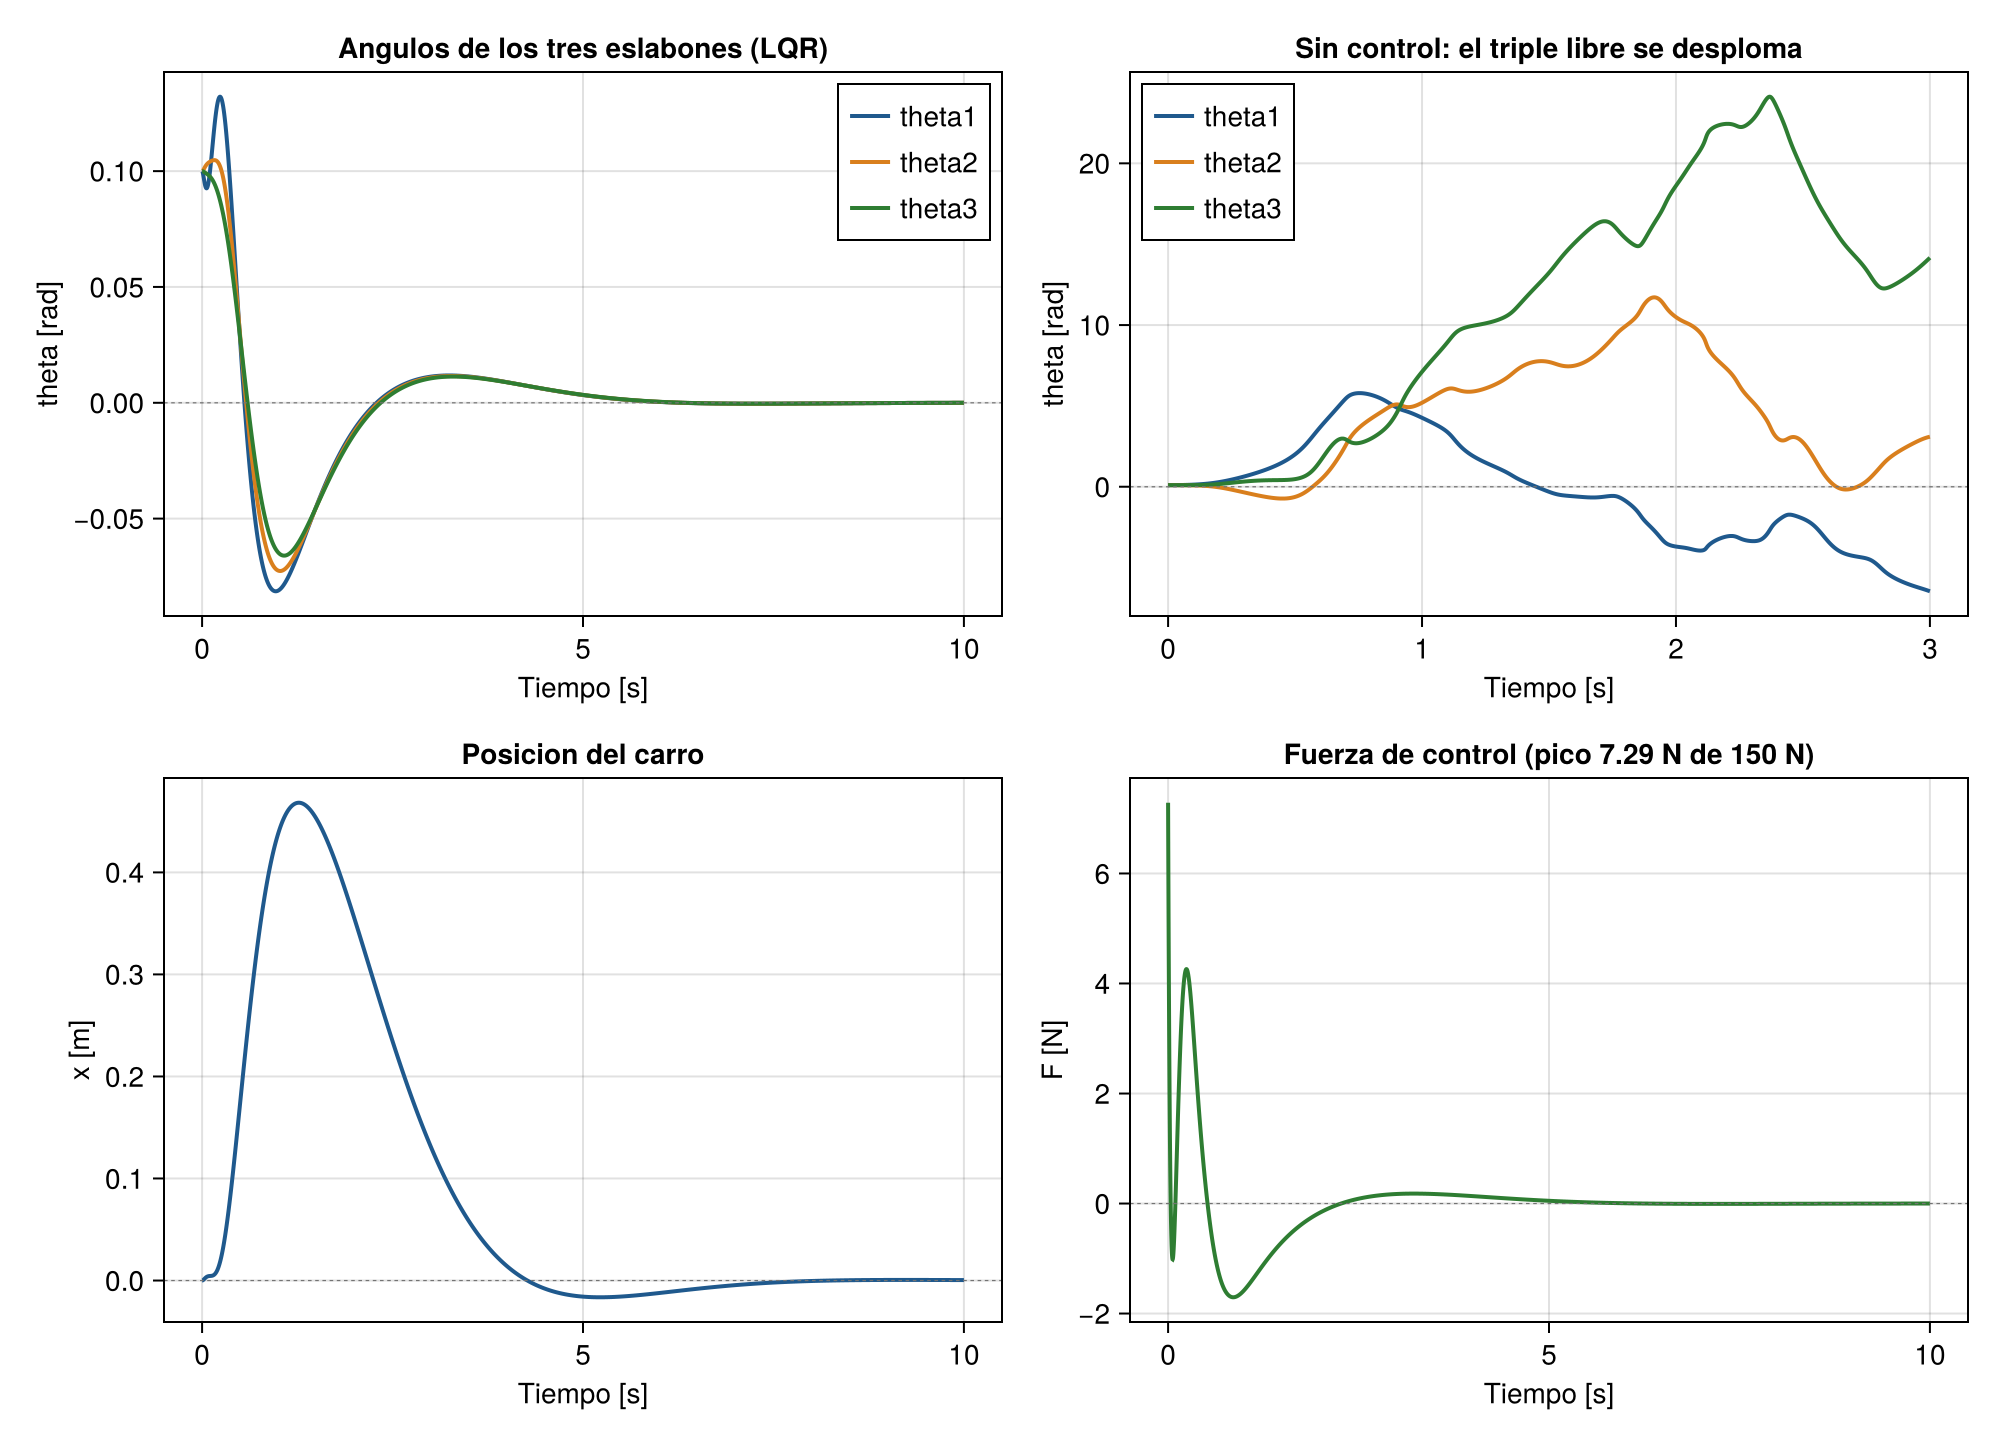
\includegraphics[width=\linewidth]{triple_respuesta.png}
  \caption{Configuración~III en lazo cerrado, desde $\theta_j=0.10$~rad en los
  tres eslabones. Arriba a la derecha, la respuesta libre: el triple sin control
  da varias vueltas completas en tres segundos. Los tiempos de asentamiento son
  1.84, 1.86 y 1.87~s con un pico de fuerza de 7.29~N.}
  \label{fig:tripleresp}
\end{figure}

\begin{figure}[htbp]
  \centering
  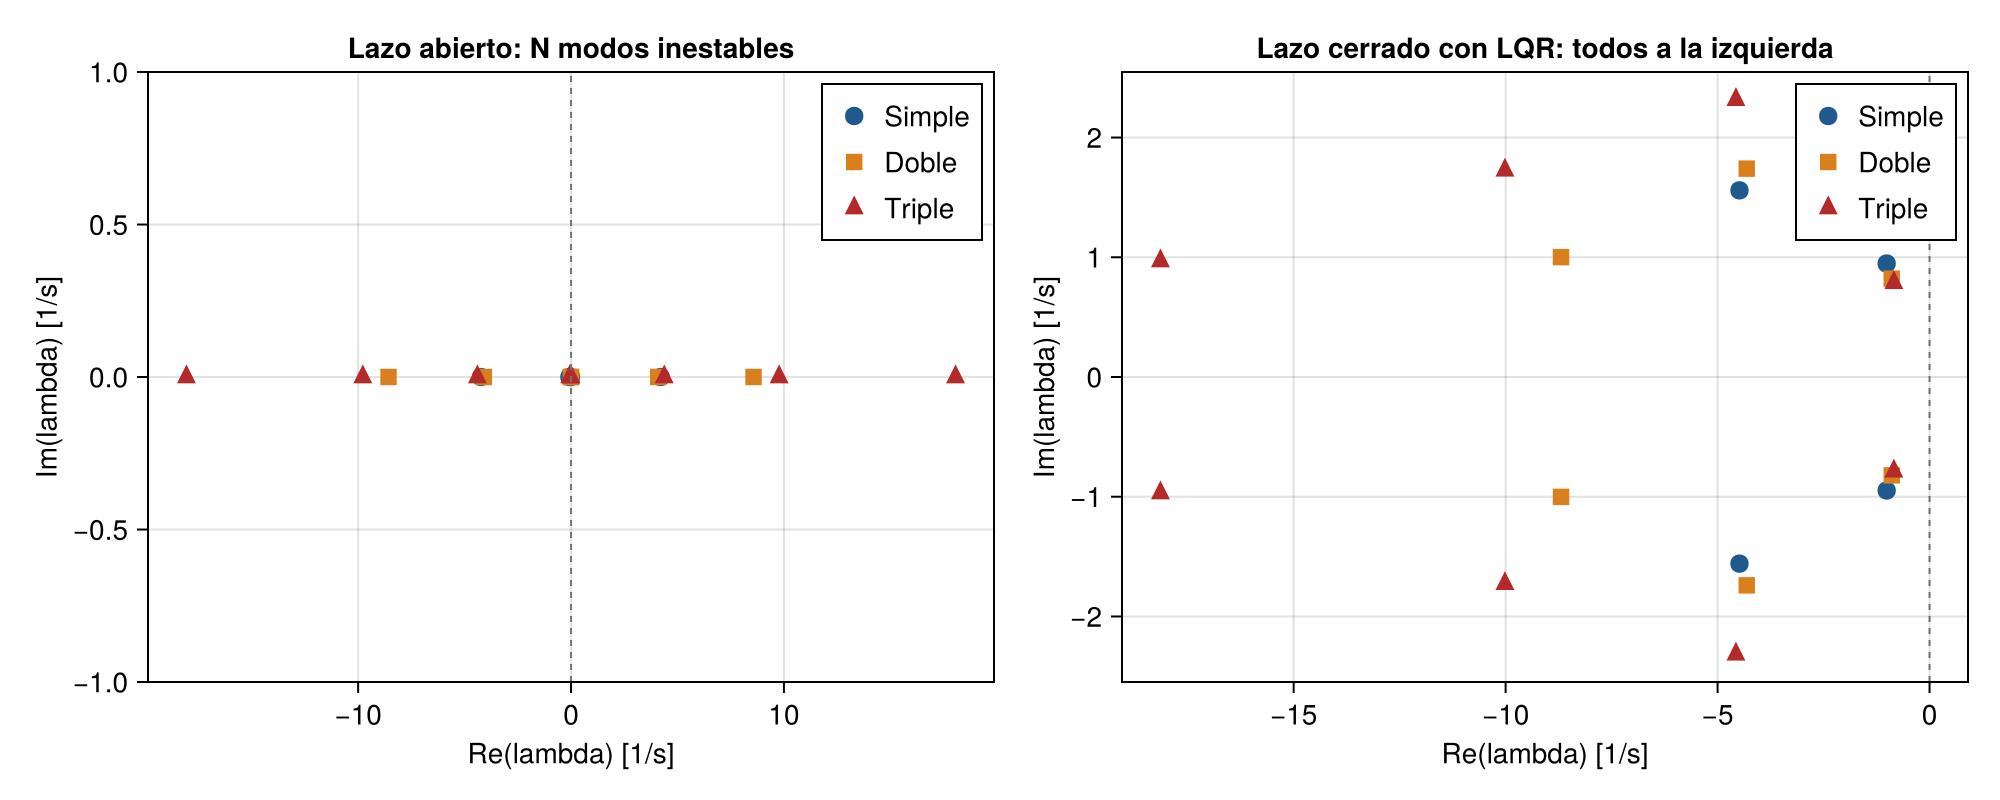
\includegraphics[width=\linewidth]{espectros_tres.png}
  \caption{Espectros de las tres configuraciones. A la izquierda, lazo abierto:
  el número de modos inestables coincide con el número de eslabones, como
  predice la \cref{prop:espectro}. A la derecha, lazo cerrado con LQR: todos los
  polos pasan al semiplano izquierdo.}
  \label{fig:espectros}
\end{figure}

% ============================================================
\section{Cuando el rango deja de servir}
\label{sec:condicionamiento}

\subsection{El problema}

El criterio de Kalman afirma que $(A,B)$ es controlable si y solo si
$\rank\calC=n$, donde $\calC$ es la matriz de controlabilidad
$[B\ \ AB\ \cdots\ A^{n-1}B]$. Es un teorema correcto.
El problema es que $\calC$ es una \emph{base de Krylov}, notoriamente mal
condicionada~\cite{golub2013}: sus columnas tienden a alinearse con el
eigenvector dominante de $A$ a medida que crece la potencia. El número de
condición que se reporta aquí es $\kappa_2=\sigma_{\max}/\sigma_{\min}$, el
cociente de valores singulares extremos~\cite{olver2018}.

Midiendo sobre la familia normalizada (longitud total 1~m, masa total 0.6~kg
repartidas en $N$ barras uniformes, $M=1$~kg, $b=0.1$), que permite comparar $N$
contra $N$ de forma limpia, se obtiene la \cref{tab:degradacion}.

\begin{table}[htbp]
  \centering\small
  \caption{Degradación con el número de eslabones. Familia normalizada.
  \textsc{Ojo:} esta familia \emph{no} coincide con los parámetros por defecto
  de las Configuraciones I y II, que tienen otras masas; es una serie aparte,
  construida para que la comparación entre valores de $N$ sea limpia.}
  \label{tab:degradacion}
  \begin{tabular}{@{}cccccc@{}}
    \toprule
    $N$ & $n$ & $\lambda_{\max}$ [s$^{-1}$] & $\hat\mu$ (PBH) & $\operatorname{cond}\calC$ & $\|K\|_2$\\
    \midrule
    1 & 4  & 4.51  & $1.31\times10^{-2}$ & $4.8\times10^{1}$  & 52.9\\
    2 & 6  & 10.59 & $1.79\times10^{-3}$ & $6.2\times10^{4}$  & 248.7\\
    3 & 8  & 18.06 & $4.92\times10^{-4}$ & $2.2\times10^{8}$  & 1176.0\\
    4 & 10 & 26.54 & $1.90\times10^{-4}$ & $1.7\times10^{12}$ & 5266.8\\
    5 & 12 & 35.64 & $9.03\times10^{-5}$ & $3.3\times10^{16}$ & 23221.9\\
    \bottomrule
  \end{tabular}
\end{table}

\begin{alerta}
\small
\textbf{Con $N=5$ el condicionamiento alcanza $1/\varepsilon_{\text{máq}}$.} En
ese punto el rango numérico de $\calC$ es \emph{ruido}: la respuesta que da el
computador no depende ya de la matemática del problema sino del redondeo. Y sin
embargo el sistema \emph{sigue siendo} controlable en aritmética exacta. Esta
tabla, por sí sola, muestra experimentalmente por qué el criterio de rango,
siendo un teorema correcto, es un mal algoritmo.
\end{alerta}

\begin{figure}[htbp]
  \centering
  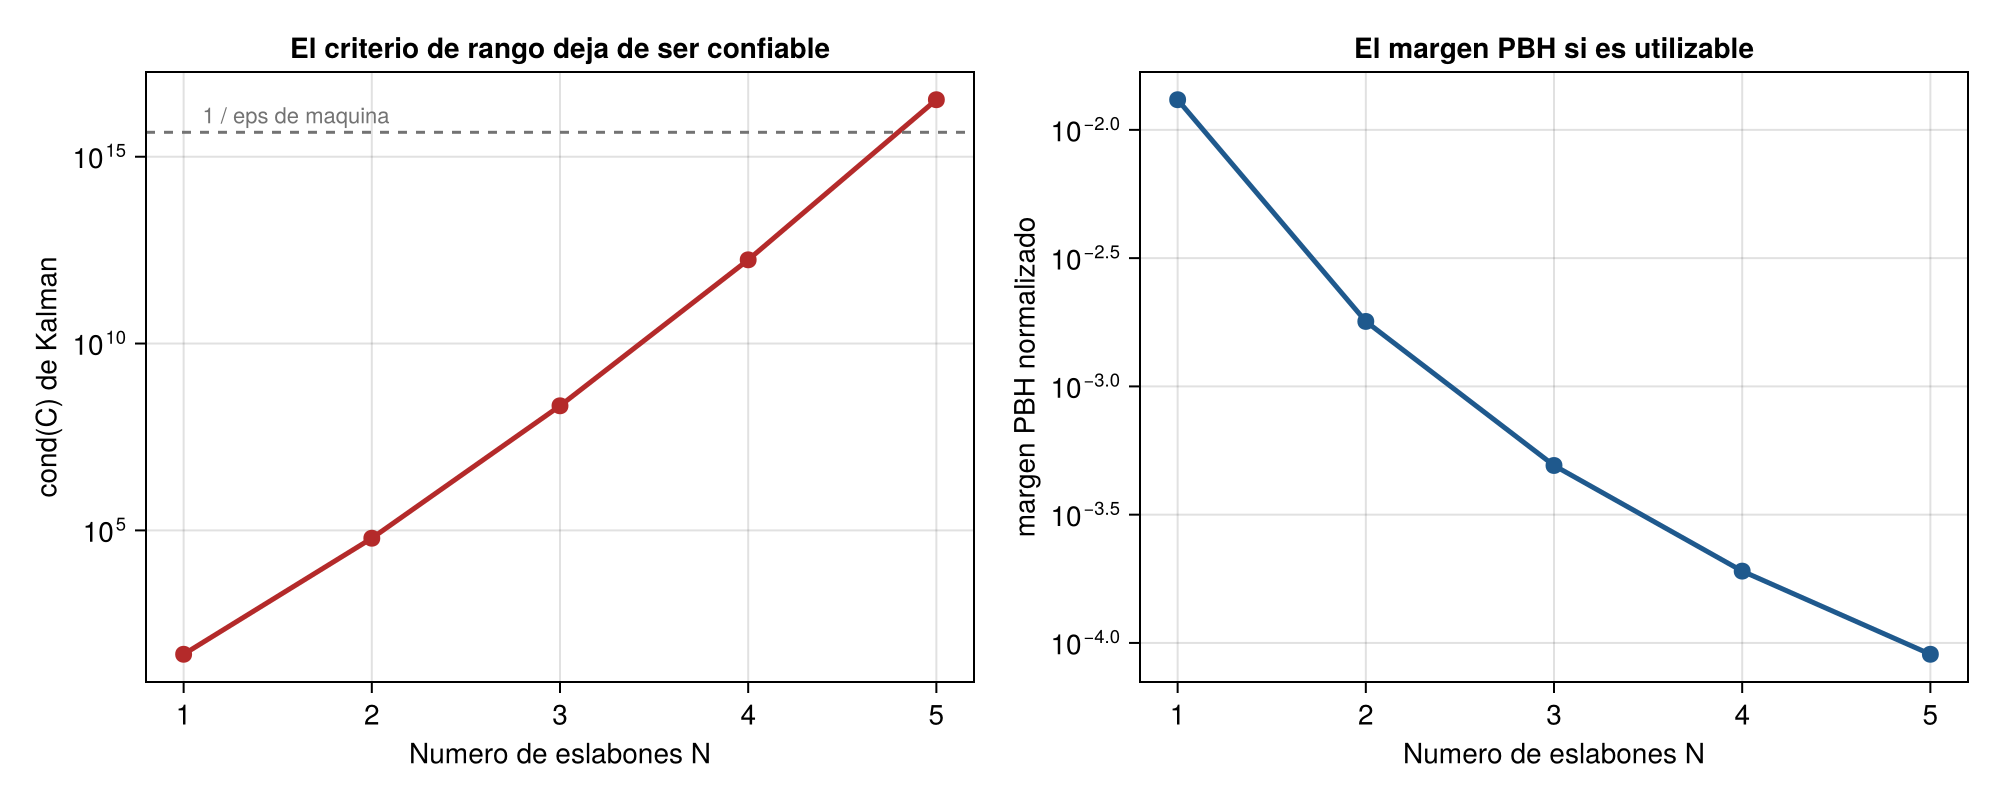
\includegraphics[width=\linewidth]{degradacion_N.png}
  \caption{Izquierda: el condicionamiento de la matriz de Kalman crece catorce
  órdenes de magnitud entre $N=1$ y $N=5$, cruzando el umbral de
  $1/\varepsilon_{\text{máq}}$. Derecha: el margen PBH decae suavemente, apenas
  dos órdenes y medio, y sigue siendo utilizable.}
  \label{fig:degradacion}
\end{figure}

\subsection{El margen de Popov--Belevitch--Hautus}
\label{sec:pbh}

La herramienta que reemplaza al rango es el test PBH en su versión cuantitativa.

\begin{teorema}[Test PBH~\cite{chen1999}]
El par $(A,B)$ es controlable si y solo si
\[
\rank\big[\,A-\lambda I\ \big|\ B\,\big]=n\qquad\text{para todo }\lambda\in\C,
\]
y basta comprobarlo en $\lambda\in\spec(A)$, pues fuera del espectro
$A-\lambda I$ ya tiene rango $n$ por sí sola.
\end{teorema}

La versión \emph{cuantitativa} sustituye el rango por el menor valor singular:
\begin{equation}
\mu_{\text{PBH}}=\min_{\lambda\in\spec(A)}\ \sigma_{\min}\big[\,A-\lambda I\ \big|\ B\,\big].
\label{eq:pbh}
\end{equation}

Esto ya no es binario. Por el teorema de Eckart--Young~\cite{eckart1936}
---en la forma en que lo enuncia \cite[Thm.~2.4.8]{golub2013}---,
$\sigma_{\min}$ de una matriz es exactamente su distancia en norma 2 al conjunto
de matrices de rango deficiente; por tanto $\mu_{\text{PBH}}$ mide \emph{cuánto habría que perturbar
el sistema para volverlo incontrolable}. Un margen pequeño significa que el
sistema es controlable ``por poco''. Para comparar entre configuraciones de
distinta escala se normaliza:
\begin{equation}
\hat\mu=\frac{\mu_{\text{PBH}}}{\big\|[\,A\ \ B\,]\big\|_2}.
\label{eq:pbhnorm}
\end{equation}

\begin{observacion}[Alcance de la métrica]
Evaluar el mínimo solo sobre $\spec(A)$ da una cota \emph{superior} de la
verdadera distancia a la incontrolabilidad de Eising~\cite{eising1984},
$\mu_E=\min_{s\in\C}\sigma_{\min}[A-sI\mid B]$, cuyo mínimo puede caer fuera del
espectro. Para comparar configuraciones la versión sobre el espectro es
suficiente y cuesta solo $n$ descomposiciones en valores singulares.
\end{observacion}

Un subproducto útil: desglosando \cref{eq:pbh} por eigenvalor se identifica
\emph{cuál} modo es el cuello de botella. En las tres configuraciones el mínimo
se alcanza en el modo inestable más rápido. Es decir, la dirección más cercana a
perderse es exactamente la que hay que controlar.

% ============================================================
\section{Dos garantías duras de álgebra lineal}

\subsection{El elipsoide de no saturación}
\label{sec:elipsoide}

Con $V(\xv)=\xv^\top P\xv$ la función de Lyapunov del LQR y $\uv=-K\xv$ ---donde
$P$, solución de la ecuación algebraica de Riccati~\cite{ogata2010}, es simétrica
definida positiva, de modo que $V$ es una forma cuadrática con mínimo único en el
origen~\cite{olver2018}---, el mayor conjunto de nivel
$\calE_c=\{\xv:\xv^\top P\xv\le c\}$ contenido en la franja de no saturación
$\{|K\xv|\le u_{\max}\}$ se obtiene resolviendo
\[
\max_{\xv^\top P\xv\le c}|K\xv|=\sqrt{c\;KP^{-1}K^\top}\ \le\ u_{\max}
\qquad\Longrightarrow\qquad
\boxed{\ c^\star=\frac{u_{\max}^2}{KP^{-1}K^\top}\ }
\]
El paso central es que el máximo de una forma lineal sobre un elipsoide es su
norma dual, un ejercicio de Cauchy--Schwarz. Dentro de $\calE_{c^\star}$ el
control \emph{nunca satura} y, para el sistema lineal,
$\dot V=-\xv^\top(Q+K^\top RK)\xv<0$, de modo que el elipsoide es invariante y
toda trayectoria que empieza dentro converge.

Como $K=R^{-1}B^\top P$, la expresión se simplifica a
$KP^{-1}K^\top=R^{-1}B^\top PBR^{-1}$, que para $R$ escalar es $B^\top PB/R^2$:
no hace falta invertir $P$. Particularizando a $\xv_0=\theta_0\bm{e}_3$ se
obtiene $|\theta_0|\le\sqrt{c^\star/P_{33}}$.

\begin{alerta}
\small
\textbf{Honestidad sobre el alcance.} $\calE_{c^\star}$ garantiza no saturación
y convergencia \emph{del sistema lineal}. Para el sistema no lineal haría falta,
además, acotar el residuo de la linealización~\cite{khalil2002}. Presentar
$c^\star$ como si fuera
la región de atracción no lineal sería un error. En la \cref{sec:atlas} se
muestra exactamente dónde y por qué la cota deja de valer.
\end{alerta}

\subsection{Discretización exacta y criterio de Schur}
\label{sec:zoh}

Todo controlador real se implementa en un computador que muestrea. Suponiendo
que la entrada se mantiene constante en cada intervalo de duración $h$
(retenedor de orden cero), la solución exacta de la EDO lineal da
\[
A_d=e^{Ah},\qquad B_d=\Big(\int_0^h e^{A\tau}d\tau\Big)B.
\]
Ambas se obtienen de \emph{una sola} exponencial matricial mediante el truco de
Van Loan~\cite{vanloan1978}: construyendo la matriz aumentada de tamaño
$(n+m)\times(n+m)$
\[
\widetilde M=\begin{pmatrix}A&B\\0&0\end{pmatrix}
\qquad\Longrightarrow\qquad
e^{\widetilde M h}=\begin{pmatrix}A_d&B_d\\0&I\end{pmatrix},
\]
de modo que $A_d$ y $B_d$ se leen directamente de los bloques superiores. Esto
evita integrar numéricamente y evita invertir $A$, que aquí sería singular
porque el carro aporta un eigenvalor nulo. La exponencial la evalúa la
biblioteca por escalamiento y cuadratura con aproximantes de
Padé~\cite[Alg.~9.3.1]{golub2013}; la implementación reproduce $e^{Ah}$ y la
integral a precisión de máquina: el error contra una serie de Taylor de orden 20
en aritmética de precisión extendida es $0$ en $A_d$ y $3.5\times10^{-18}$ en
$B_d$.

La condición de estabilidad en tiempo discreto es que $A_d-B_dK$ sea de
\emph{Schur}, es decir que todos sus eigenvalores estén dentro del círculo
unitario. Es el análogo discreto de la condición de Hurwitz
$\Real\lambda_i<0$~\cite[Thm.~10.16]{olver2018}, y sale de que la solución
discreta es $\xv_k=(A_d-B_dK)^k\xv_0$.

\begin{observacion}[Dos formulaciones distintas del control cuadrático]
Conviene no confundir el regulador de este trabajo con la otra formulación
cuadrática habitual. Aquí el problema es de \emph{horizonte infinito} y en
tiempo continuo: la ganancia $K$ es estacionaria y sale de la ecuación de
Riccati. La alternativa, natural una vez discretizado el sistema, es el problema
de \emph{horizonte finito} sobre $t=1,\dots,T$, que no produce una ganancia de
realimentación sino una secuencia de entradas, y que se resuelve apilando
estados y entradas en un único problema de mínimos cuadrados con restricciones
lineales~\cite[\S17.2]{boyd2018}. Misma función de costo, dos objetos
matemáticos distintos.
\end{observacion}

% ============================================================
\section{El atlas de operabilidad}
\label{sec:atlas}

\subsection{Dos tipos de imposibilidad}

La pregunta ``¿dónde funciona el controlador?'' admite dos respuestas de
naturaleza distinta, y el informe debe separarlas:

\begin{itemize}
  \item \textbf{Imposibilidad estructural.} El par $(A,B)$ deja de ser
  controlable, o se acerca tanto que ningún $K$ razonable sirve. Es una
  propiedad \emph{del sistema}, independiente del controlador. Se mide con el
  margen PBH.
  \item \textbf{Imposibilidad práctica.} El sistema es controlable, pero el
  actuador satura, el riel se acaba o el muestreo es demasiado lento. Es una
  propiedad \emph{de la implementación}. Se mide integrando el modelo no lineal
  y buscando la frontera por bisección.
\end{itemize}

El criterio de éxito, del que depende toda frontera práctica, se fija así:
\[
\text{éxito}\iff\Big(\max_j|\theta_j(T)|<0.02\ \text{rad}\Big)\wedge\Big(\max_t|x(t)|\le x_{\text{riel}}\Big)\wedge\Big(\max_{t,j}|\theta_j(t)|<\pi/2\Big)
\]
con $T=10$~s y $x_{\text{riel}}=1.5$~m. El umbral de 0.02~rad es el mismo que
define el tiempo de asentamiento en la primera entrega: se reutiliza en lugar de
inventar otro.

\begin{observacion}[La bisección está bien planteada]
La bisección sobre $\theta_0$ supone que el conjunto de recuperación es un
intervalo: si el sistema se recupera desde $\theta_0$, se recupera desde
cualquier ángulo menor. Si hubiera huecos, el resultado no significaría nada. Se
verificó sobre las 130 filas de las mallas calculadas: \emph{cero huecos}.
\end{observacion}

\subsection{La frontera de operabilidad}

\begin{figure}[htbp]
  \centering
  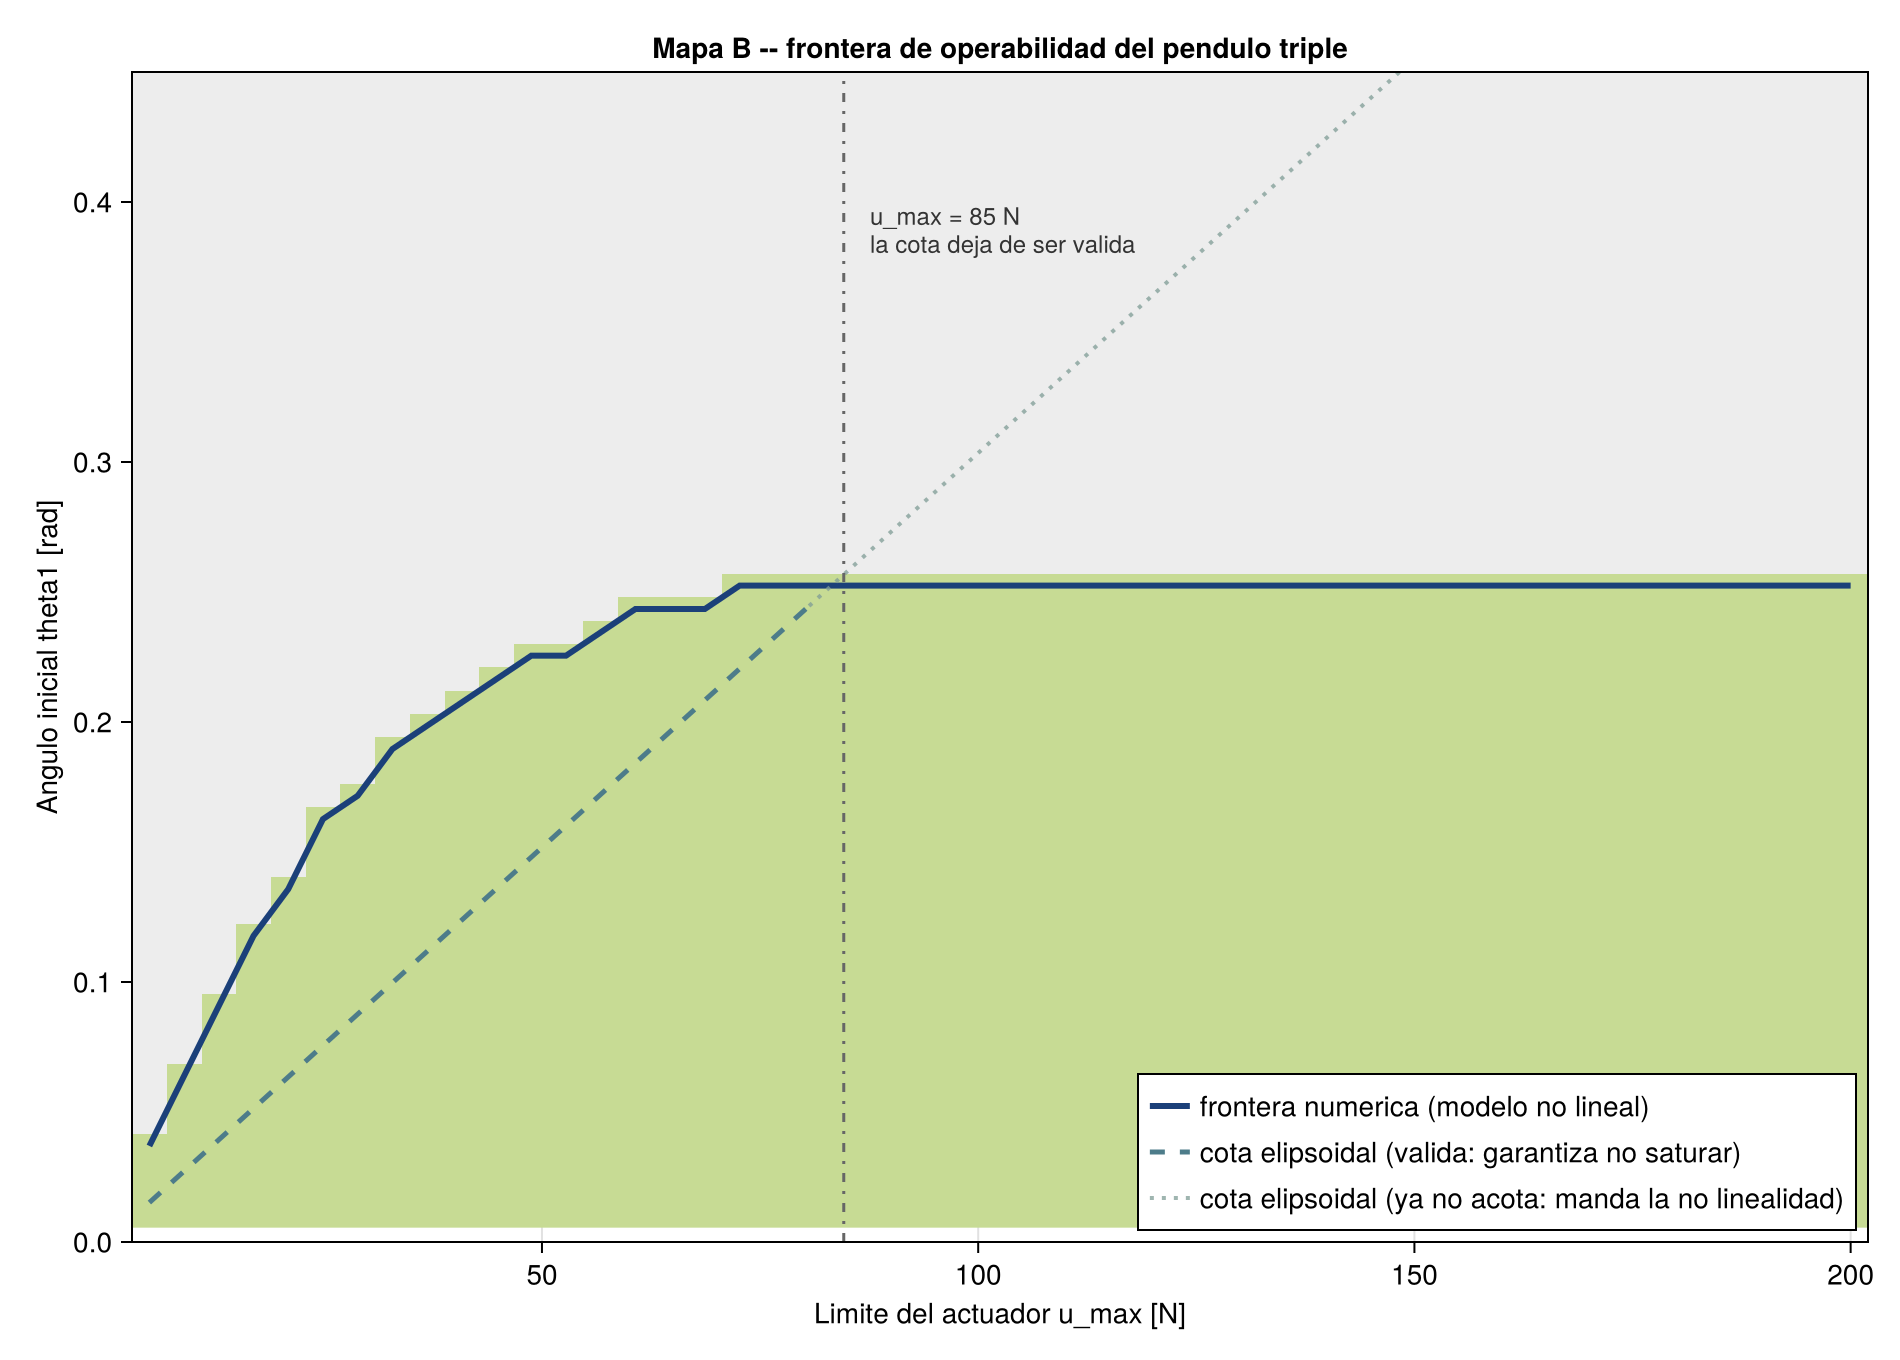
\includegraphics[width=0.92\linewidth]{atlas_b.png}
  \caption{Frontera de operabilidad de la Configuración~III en el plano
  $(u_{\max},\theta_0)$. La zona clara es donde el controlador recupera. La
  curva continua es la frontera numérica sobre el modelo no lineal; la línea
  segmentada es la cota elipsoidal $\theta_0=\sqrt{c^\star/P_{33}}$, que por ser
  $c^\star\propto u_{\max}^2$ resulta \emph{lineal} en $u_{\max}$.}
  \label{fig:atlasb}
\end{figure}

La \cref{fig:atlasb} concentra tres resultados:

\begin{enumerate}
  \item \textbf{La cota elipsoidal es conservadora y válida ---hasta cierto
  punto.} Para $u_{\max}\le85$~N queda por dentro de la frontera numérica, como
  debe ser. Con $u_{\max}=50$~N garantiza $0.152$~rad frente a los $0.230$~rad
  reales: un $66\%$ de la frontera.

  \item \textbf{Más allá de 85~N la cota deja de acotar.} Como $c^\star$ crece
  con $u_{\max}^2$, la cota crece linealmente y sin límite; pero la frontera
  real se estanca. La razón es precisamente la advertencia de la
  \cref{sec:elipsoide}: $c^\star$ certifica no saturación más convergencia
  \emph{lineal}, y una vez que la saturación deja de ser la restricción activa,
  lo que limita es la no linealidad, sobre la que $c^\star$ no dice nada.

  \item \textbf{Más actuador deja de comprar ángulo a partir de unos 73~N.} La
  frontera crece hasta $0.252$~rad y desde ahí se mantiene plana en todo el
  resto del barrido, hasta 200~N. Pasado ese punto, comprar un motor más grande
  no amplía la región de operación: la restricción activa ha dejado de ser el
  actuador. Nótese que ocurre \emph{antes} del cruce del punto anterior, y en
  ese orden: primero la saturación deja de mandar (73~N) y solo después la cota
  elipsoidal ---que sigue creciendo linealmente--- alcanza y rebasa a la
  frontera (85~N).
\end{enumerate}

\subsection{Cuál restricción está activa}

Separando cada límite se descubre que \emph{la restricción activa cambia con la
configuración}, lo que obliga a matizar la clasificación anterior: la
imposibilidad práctica no es un bloque homogéneo.

\begin{table}[htbp]
  \centering\small
  \caption{Frontera práctica por configuración, con $u_{\max}=50$~N. La columna
  ``sin riel'' repite el cálculo eliminando la restricción de carrera. La cota
  $c^\star$ debe compararse contra esa columna, no contra la nominal.}
  \label{tab:restricciones}
  \begin{tabular}{@{}lcccc@{}}
    \toprule
    \textbf{Config.} & \textbf{cota} $c^\star$ [rad] & \textbf{frontera} [rad] & \textbf{sin riel} [rad] & \textbf{restricción activa}\\
    \midrule
    Simple & 0.962 & 0.580 & 1.063 & \textbf{riel} (1.5 m)\\
    Doble  & 0.234 & 0.345 & 0.345 & saturación\\
    Triple & 0.152 & 0.230 & 0.230 & saturación\\
    \bottomrule
  \end{tabular}
\end{table}

En el péndulo simple el carro alcanza exactamente 1.500~m con
$\theta_0=0.5798$~rad y 1.574~m con $\theta_0=0.60$: el fallo es
\emph{únicamente} por carrera, con el ángulo convergiendo perfectamente y el
motor al $54\%$ de su capacidad. En el doble y el triple el riel nunca llega a
morder. Comparada contra la columna correcta, la cota elipsoidal queda por
dentro en las tres configuraciones, con un conservadurismo del $90\%$, $68\%$ y
$66\%$ respectivamente.

\subsection{Dónde funciona mejor: un óptimo interior}

\begin{figure}[htbp]
  \centering
  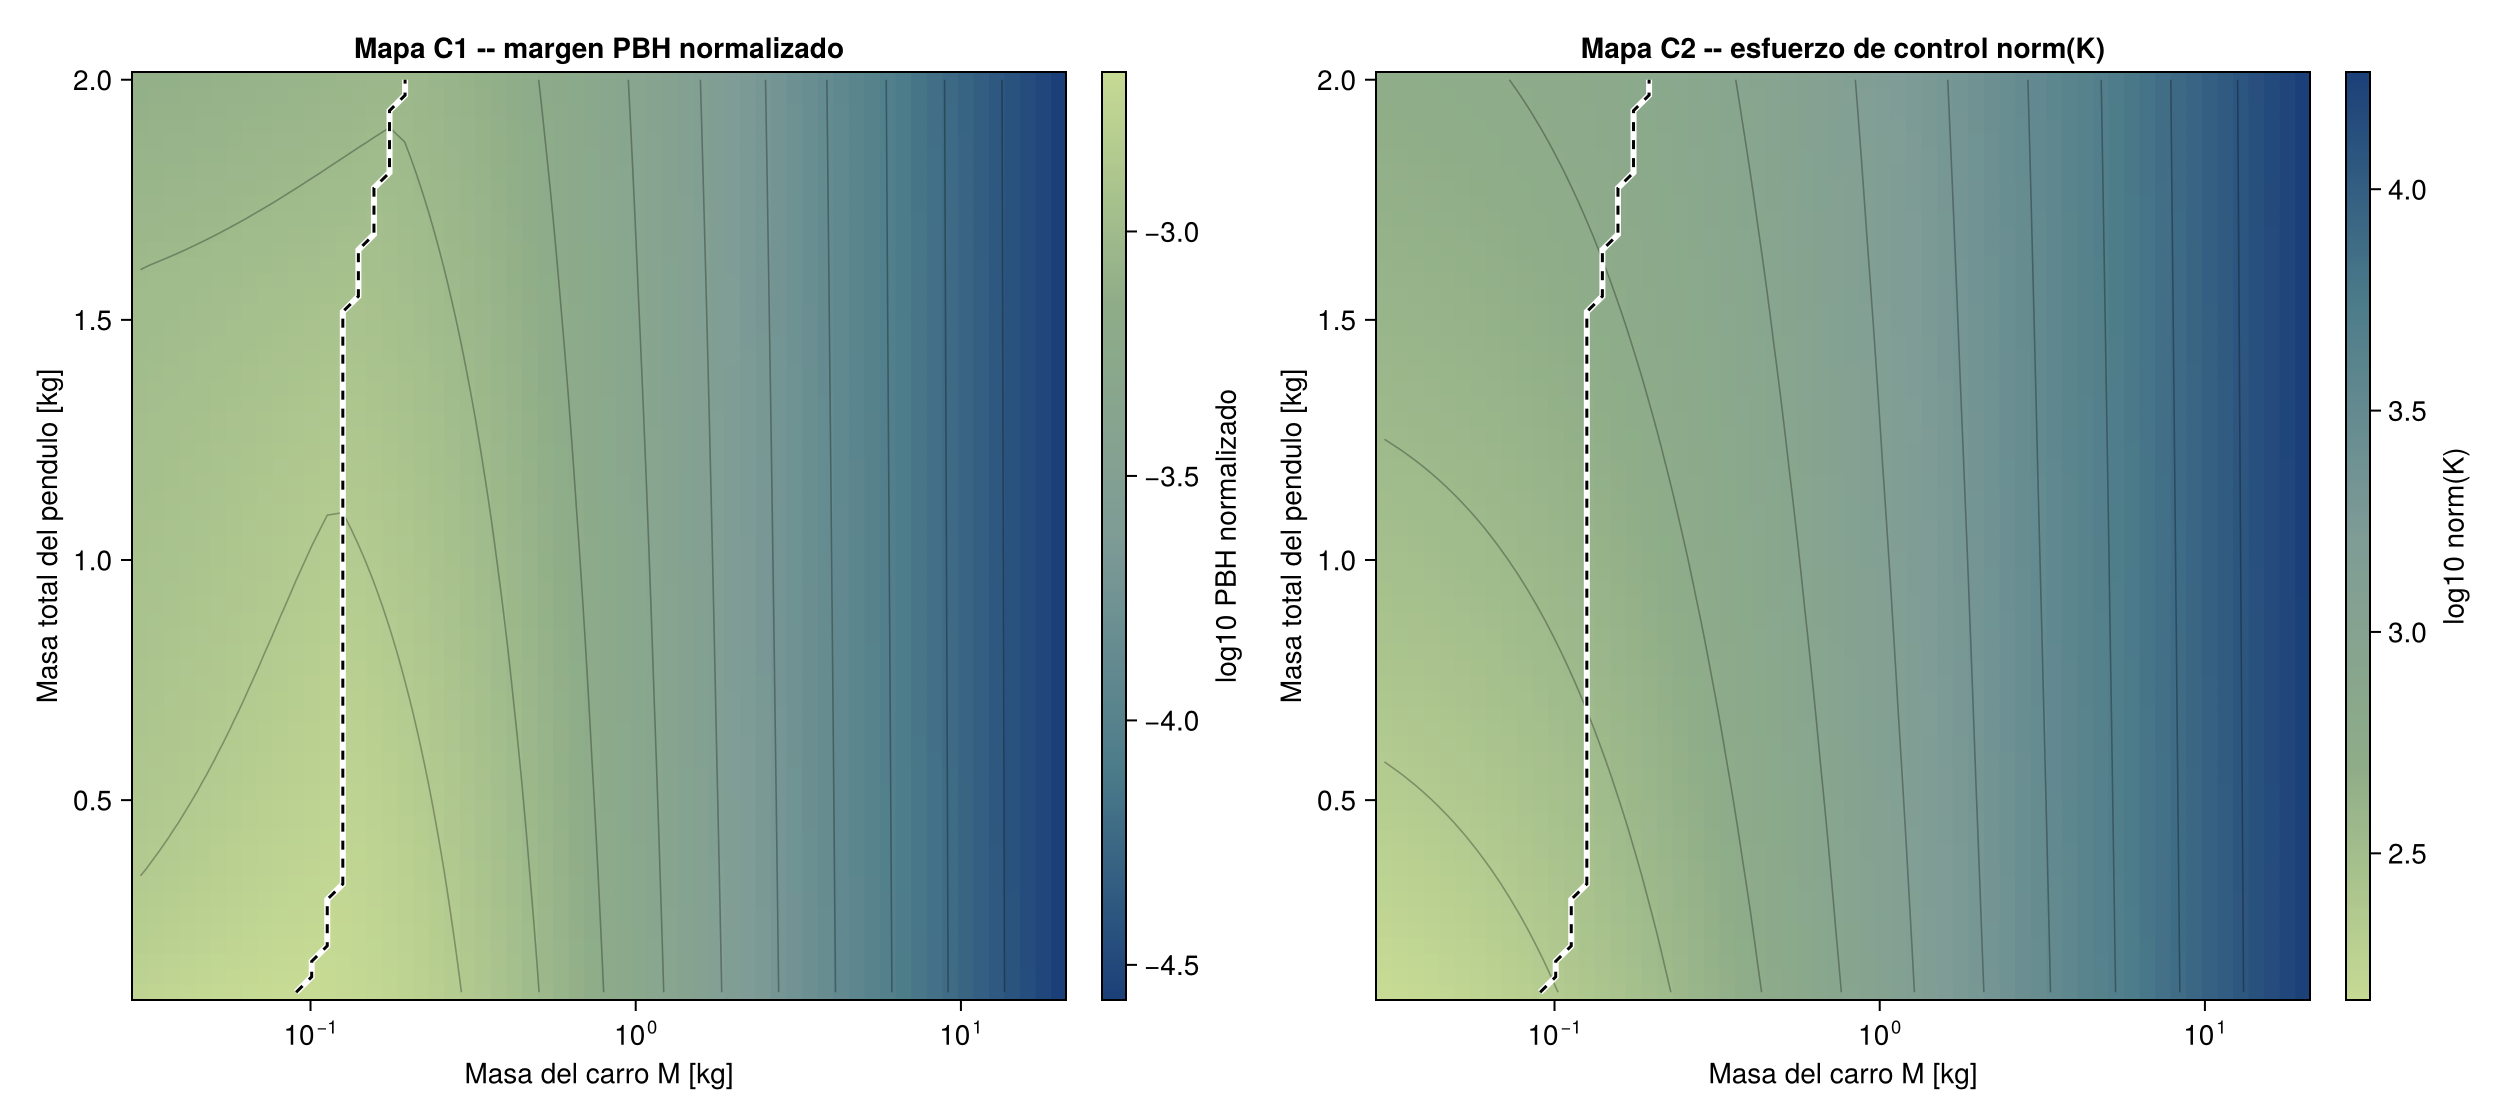
\includegraphics[width=\linewidth]{atlas_c.png}
  \caption{Mapa de la masa del carro contra la masa total del péndulo. La línea
  segmentada marca, para cada masa de péndulo, la masa de carro que maximiza el
  margen PBH. En ambos paneles el color claro es ``mejor''. El óptimo del margen
  \emph{no} coincide con el del esfuerzo de control, que es monótono.}
  \label{fig:atlasc}
\end{figure}

El barrido de la masa del carro produce el resultado más interesante del atlas:
\textbf{el margen PBH no es monótono, sino que tiene un máximo interior} en
$M\approx0.126$~kg. La interpretación es un compromiso: un carro muy pesado se
mueve poco ante la misma fuerza y pierde autoridad de control ($\|K\|$ crece
hasta 18\,043 con $M=20$~kg), mientras que uno muy liviano se mueve mucho pero
degrada el acoplamiento con los eslabones. En medio hay un óptimo.

Nótese además que $c^\star$ y $\hat\mu$ \emph{apuntan en direcciones opuestas} en
este barrido: $c^\star$ crece monótonamente con $M$ mientras que $\hat\mu$ tiene
un máximo. No existe una única ``mejor'' configuración; depende de qué se
optimice.

\begin{figure}[htbp]
  \centering
  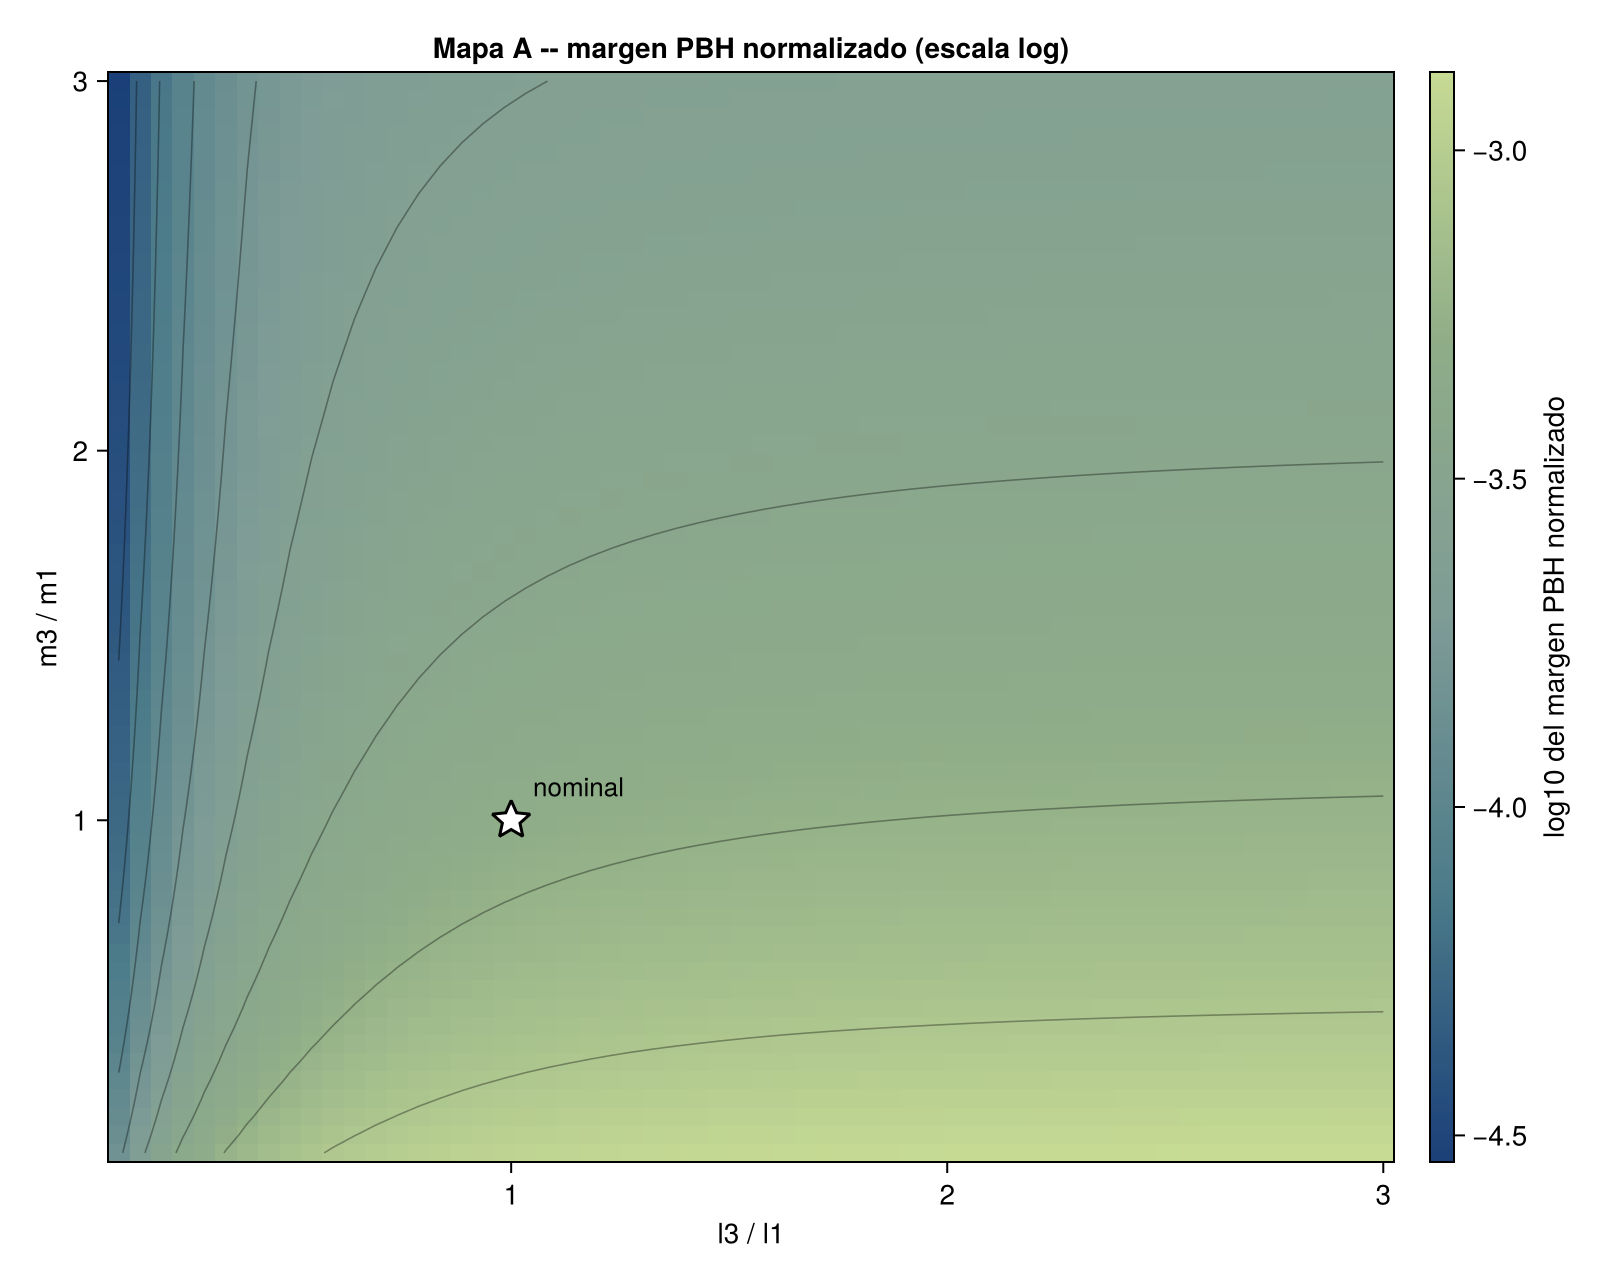
\includegraphics[width=0.86\linewidth]{atlas_a.png}
  \caption{Región estructuralmente sana en el plano de las razones geométricas
  del eslabón superior. La estrella marca la configuración nominal
  ($\ell_3/\ell_1=m_3/m_1=1$). El margen es máximo abajo a la derecha: eslabón
  superior \emph{largo} y \emph{ligero}. Ambos efectos van en el mismo sentido,
  pero el de la longitud es el dominante: a masa nominal, pasar de
  $\ell_3/\ell_1=0.1$ a $3$ multiplica el margen por $10.6$, mientras que a
  longitud máxima, aligerar de $m_3/m_1=3$ a $0.1$ lo multiplica por $5.0$.}
  \label{fig:atlasa}
\end{figure}

Los barridos geométricos confirman una intuición conocida y la cuantifican
(\cref{fig:atlasa}): el eslabón superior \emph{corto} es el peligroso. Con
$\ell_3=2$~cm el modo dominante sube a $42.9$~s$^{-1}$ y el margen PBH cae a
$3.4\times10^{-5}$; alargarlo hasta 2~m lo baja a $17.3$~s$^{-1}$ y sube el
margen a $6.0\times10^{-4}$. Es el efecto de la escoba larga en la palma de la
mano, ahora medido y en la punta de un péndulo triple.

\subsection{Sobre el peso del control}

\begin{figure}[htbp]
  \centering
  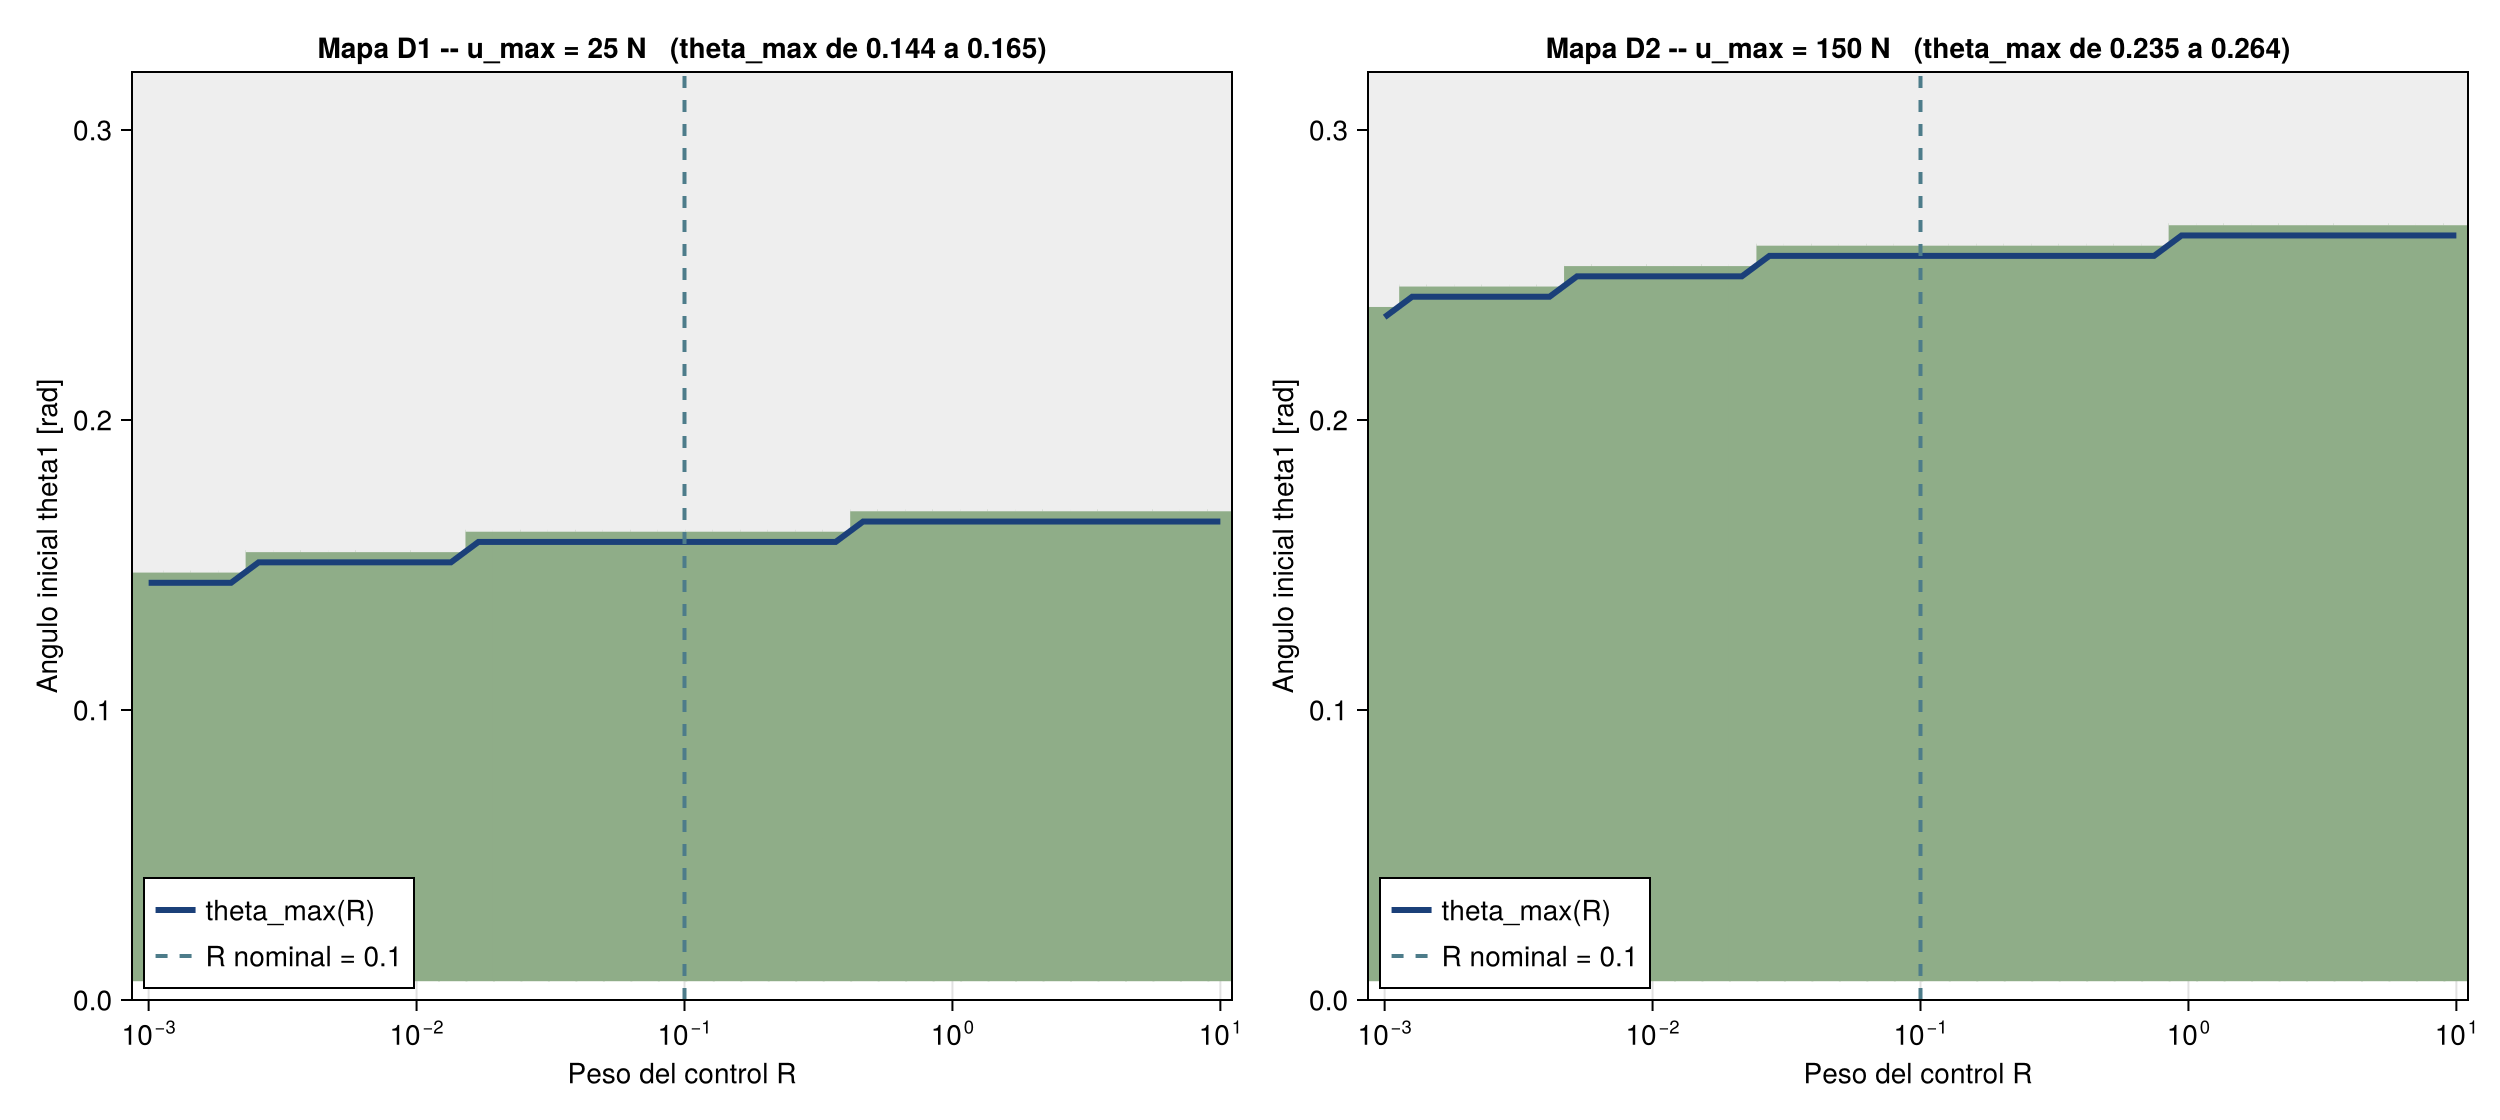
\includegraphics[width=\linewidth]{atlas_d.png}
  \caption{Ángulo recuperable en función del peso $R$ del control, para un
  actuador limitado (izquierda) y uno holgado (derecha).}
  \label{fig:atlasd}
\end{figure}

Cuatro órdenes de magnitud en $R$ mueven el ángulo recuperable apenas un
$11$--$13\%$, y el $R=0.1$ nominal queda a menos del $5\%$ del óptimo en ambos
regímenes. Más llamativo aún: $\|K\|$ varía solo un factor $2$ (de 2197 a 1053)
sobre ese mismo rango.

La razón es estructural. La planta es tan inestable que cualquier $K$ que
estabilice debe cancelar tres modos con parte real de hasta $+18.06$, y eso ya
fija la escala de la ganancia. \emph{El peso del control no puede abaratar lo
que la inestabilidad exige.} Ajustar $R$, aquí, compra muy poco.

\subsection{Muestreo}

Aplicando la bisección de la \cref{sec:zoh} sobre $h$ con criterio de Schur:

\begin{table}[htbp]
  \centering\small
  \caption{Período de muestreo máximo con los parámetros por defecto.}
  \label{tab:muestreo}
  \begin{tabular}{@{}lccc@{}}
    \toprule
    \textbf{Config.} & $h_{\max}$ [ms] & $1/\lambda_{\max}$ [ms] & $h_{\max}\lambda_{\max}$\\
    \midrule
    Simple & 197.4 & 237.5 & 0.83\\
    Doble  & 77.3  & 116.7 & 0.66\\
    Triple & 32.0  & 55.4  & 0.58\\
    \bottomrule
  \end{tabular}
\end{table}

El triple exige muestrear por encima de \textbf{31~Hz}, y el margen relativo
respecto al tiempo de caída se estrecha al crecer la complejidad
($0.83\to0.66\to0.58$): no basta con escalar la frecuencia proporcionalmente al
modo dominante.

% ============================================================
\section{Estimación de estado}
\label{sec:observador}

\subsection{La dualidad convierte el problema en uno ya resuelto}

Hasta aquí el control ha sido $\uv=-K\xv$, con el estado completo. En un sistema
real eso no se mide. Se estima con un observador de
Luenberger~\cite{ogata2010,chen1999}
\[
\dot{\hat\xv}=A\hat\xv+B\uv+L\big(\yv-C\hat\xv\big),
\]
y el error $\ev=\xv-\hat\xv$ obedece $\dot\ev=(A-LC)\ev$. Diseñar $L$ para que
$A-LC$ sea Hurwitz es el \emph{problema dual} de diseñar $K$: por la dualidad de
Kalman, $(A,B)$ controlable $\iff$ $(A^\top,B^\top)$ observable, de modo que
\begin{equation}
L=\operatorname{lqr}\!\big(A^\top,\ C^\top,\ Q_o,\ R_o\big)^{\!\top}
\label{eq:dualidad}
\end{equation}
y \emph{no hace falta escribir un solo algoritmo nuevo}: se reutiliza la misma
ecuación de Riccati resuelta por la matriz hamiltoniana. La implementación
verifica que \cref{eq:dualidad} coincide con el diseño directo hasta el último
bit.

Si además se interpretan $Q_o$ y $R_o$ como covarianzas del ruido de proceso y
de medición, $L$ es la ganancia del \emph{filtro de Kalman} en régimen
permanente, y el conjunto $K+L$ constituye un controlador LQG.

\subsection{El principio de separación}

\begin{teorema}[Principio de separación]
\label{teo:separacion}
En coordenadas $(\xv,\ev)$, el sistema en lazo cerrado con observador tiene
matriz \emph{triangular por bloques}
\[
\begin{pmatrix}\dot\xv\\ \dot\ev\end{pmatrix}=
\begin{pmatrix}A-BK & BK\\ 0 & A-LC\end{pmatrix}
\begin{pmatrix}\xv\\ \ev\end{pmatrix},
\]
y por tanto $\spec=\spec(A-BK)\cup\spec(A-LC)$.
\end{teorema}

\begin{proof}
De $\dot\xv=A\xv-BK\hat\xv=A\xv-BK(\xv-\ev)=(A-BK)\xv+BK\ev$ y
$\dot\ev=\dot\xv-\dot{\hat\xv}=A(\xv-\hat\xv)-LC(\xv-\hat\xv)=(A-LC)\ev$. El
espectro de una matriz triangular por bloques es la unión de los espectros de
sus bloques diagonales~\cite{hoffman1971}.
\end{proof}

La consecuencia es que el controlador y el observador se diseñan de forma
\emph{independiente}. Es un resultado de control que se demuestra en dos líneas
de álgebra lineal. Verificado numéricamente en las tres configuraciones, el
error máximo al emparejar espectros es de $3.4\times10^{-12}$.

Conviene notar que el bloque $(1,2)$ \emph{no} es nulo: el error de estimación sí
perturba a la planta. Lo que la triangularidad garantiza es que esa perturbación
no puede desestabilizar, porque el error decae por su cuenta.

\begin{figure}[htbp]
  \centering
  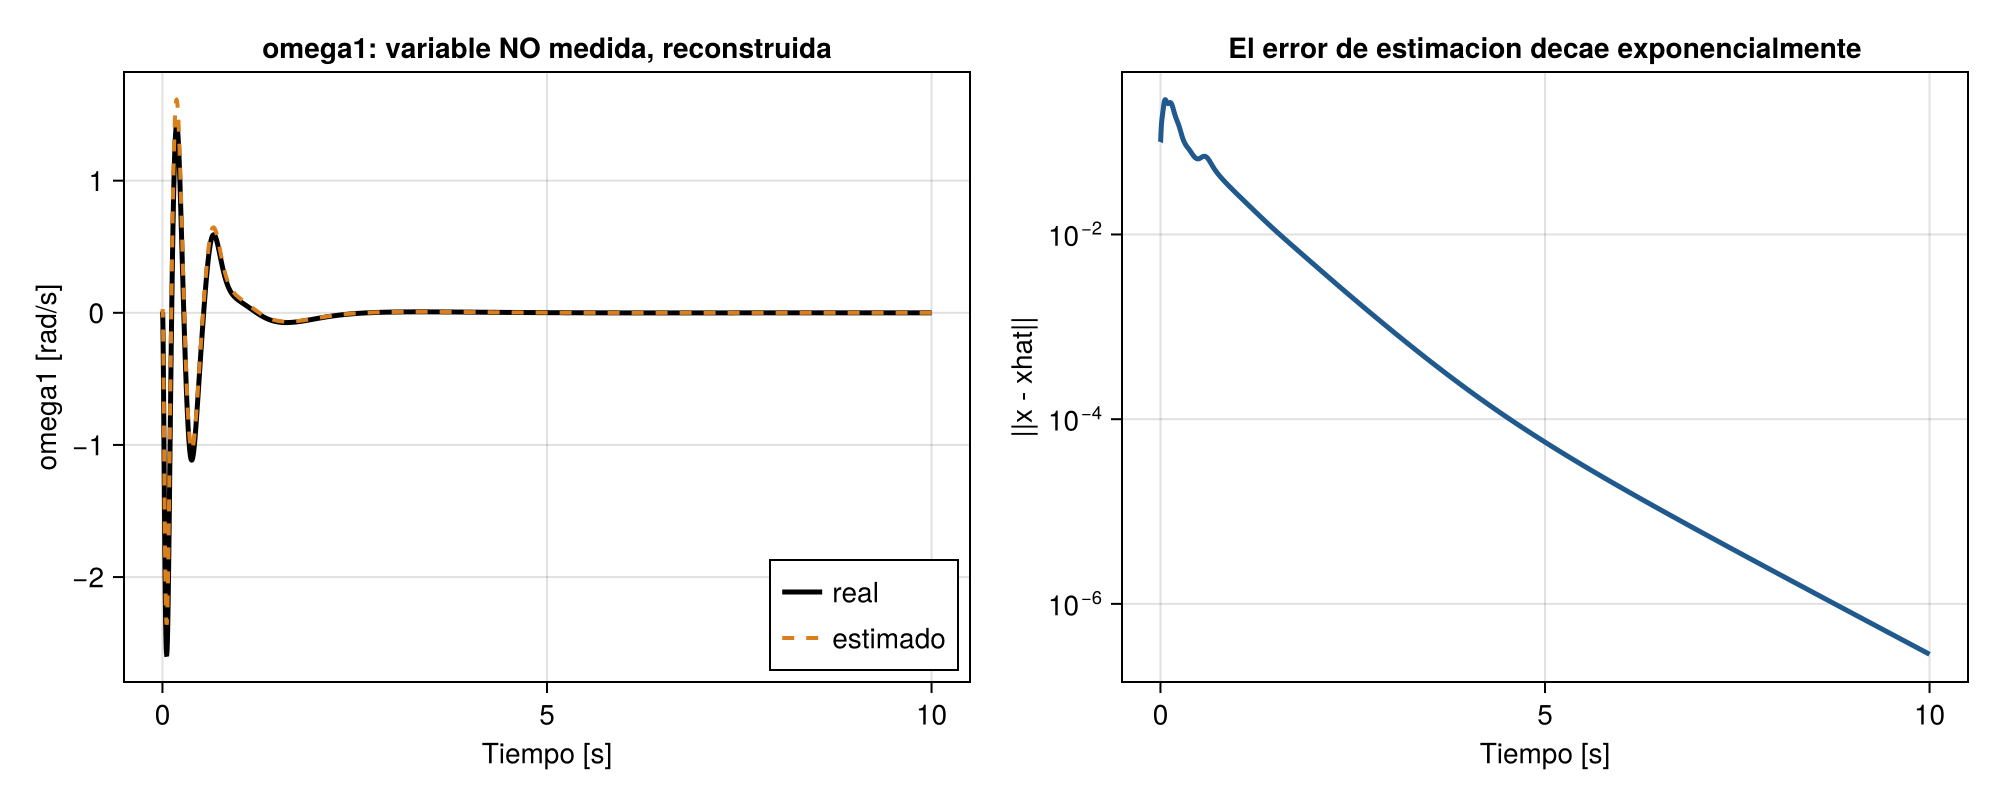
\includegraphics[width=\linewidth]{observador.png}
  \caption{Izquierda: reconstrucción de $\omega_1$, que \emph{no} se mide, a
  partir de la posición y los tres ángulos. Derecha: el error de estimación
  decae exponencialmente ---una recta en escala logarítmica--- como predice
  $\dot\ev=(A-LC)\ev$ con $A-LC$ de Hurwitz. Condición inicial:
  $\theta_1=0.10$~rad con el estimador arrancando en cero.}
  \label{fig:observador}
\end{figure}

\subsection{El precio de estimar: la región de atracción se encoge}
\label{sec:precioestimar}

El \cref{teo:separacion} garantiza la estabilidad del sistema \emph{lineal}
aumentado. No dice nada sobre la región de atracción del sistema no
lineal~\cite{khalil2002}, y ahí el precio de estimar en vez de medir resulta
considerable. Midiendo por
bisección el mayor ángulo inicial recuperable con el estimador arrancando en
cero, contra el mismo cálculo con estado completo:

\begin{table}[htbp]
  \centering\small
  \caption{Región de atracción con estado completo frente a la del lazo con
  observador, $u_{\max}=150$~N. La condición inicial desvía los primeros
  $k$ ángulos por igual.}
  \label{tab:roaobs}
  \begin{tabular}{@{}cccc@{}}
    \toprule
    \textbf{Ángulos desviados} & \textbf{estado completo} [rad] & \textbf{con observador} [rad] & \textbf{ratio}\\
    \midrule
    1 & 0.2605 & 0.1452 & 56\,\%\\
    2 & 0.1419 & 0.0450 & 32\,\%\\
    3 & 0.3018 & 0.0743 & 25\,\%\\
    \bottomrule
  \end{tabular}
\end{table}

\begin{observacion}[Por qué la columna de estado completo no es monótona]
Desviar \emph{tres} ángulos ($0.3018$~rad) resulta más benigno que desviar
\emph{uno} ($0.2605$) y mucho más que desviar \emph{dos} ($0.1419$). No es un
error de medida sino geometría: con los tres eslabones inclinados por igual, la
cadena se comporta como una única barra rígida y el problema se parece al del
péndulo simple; con dos inclinados y el tercero vertical hay un quiebre en la
articulación superior, que es la configuración más exigente. La columna de
ratios, en cambio, sí decae monótonamente, porque compara cada caso consigo
mismo.
\end{observacion}

La caída es sustancial: entre la mitad y la cuarta parte. El mecanismo, medido
sobre la simulación, resulta ser el contrario del que cabría esperar. El
estimador arranca en cero, de modo que en $t=0$ el mando también vale cero,
mientras que con estado completo vale $-K_3\theta_1=31.74$~N: durante el
transitorio inicial el controlador no aplica fuerza de más sino \emph{de menos}.
Desde la misma condición inicial su pico llega a ser \emph{menor} ---25.8~N
frente a 31.7~N desviando un ángulo $0.10$~rad, 16.4~N frente a 26.8~N desviando
dos $0.045$~rad---. Solo lo supera en la condición de tres ángulos iguales, que
es precisamente aquella en la que los signos alternos de $K$ se cancelan y el
lazo con estado completo baja a 5.4~N; el observador, que no reproduce esa
cancelación mientras estima mal, pide 16.1~N.

Lo que sí crece es la \emph{excursión}. Mientras la estimación converge ---el
error de estimación tarda 2.95~s en caer al $1\%$ de su valor inicial--- la
planta cae gobernada por un mando que todavía no la describe, y el ángulo máximo
que alcanza durante el transitorio se multiplica por un factor de entre $1.1$ y
$2.8$ según la condición inicial. Es esa sobre-excursión, y no un exceso de
esfuerzo, la que saca a la planta del régimen en que la linealización es válida;
una vez fuera, el observador lineal ya no la describe bien y el error deja de
converger. El umbral se ve nítido justo en la frontera: desde
$\theta_0=0.1452$~rad la excursión llega a $0.2211$~rad y el lazo todavía se
recupera; desde $0.1500$~rad ya no.

\begin{alerta}
\small
\textbf{Consecuencia práctica.} La condición inicial nominal de este informe
---los tres eslabones a $0.10$~rad--- está \emph{dentro} de la región de
atracción con estado completo ($0.3018$~rad) y \emph{fuera} de la del lazo con
observador ($0.0743$~rad): con estado completo converge en 1.85~s, con
observador diverge. Es un recordatorio de que el principio de separación es un
teorema sobre el sistema linealizado, y de que un diseño que solo se valide en
ese marco puede fallar en la planta real.
\end{alerta}

\subsection{Cuál es el juego mínimo de sensores}

Evaluando los $2^4-1=15$ subconjuntos no vacíos de $\{x,\theta_1,\theta_2,\theta_3\}$
se obtiene una partición limpia y total:

\begin{table}[htbp]
  \centering\small
  \caption{Observabilidad por subconjunto de sensores en la Configuración~III.}
  \label{tab:sensores}
  \begin{tabular}{@{}lcc@{}}
    \toprule
    \textbf{Sensores} & $\rank\calO$ & \textbf{margen PBH normalizado}\\
    \midrule
    $x+\theta_1+\theta_2+\theta_3$ & 8/8 & $1.58\times10^{-4}$\\
    $x+\theta_2+\theta_3$ & 8/8 & $1.45\times10^{-4}$\\
    $x+\theta_1+\theta_3$ & 8/8 & $1.12\times10^{-4}$\\
    $x+\theta_1+\theta_2$ & 8/8 & $9.96\times10^{-5}$\\
    $x+\theta_3$ & 8/8 & $9.25\times10^{-5}$\\
    $x+\theta_1$ & 8/8 & $6.29\times10^{-5}$\\
    $x+\theta_2$ & 8/8 & $1.74\times10^{-5}$\\
    $x$ & 8/8 & $1.49\times10^{-6}$\\
    \midrule
    cualquiera sin $x$ (7 casos) & 7/8 & $0$\\
    \midrule
    \multicolumn{3}{@{}l@{}}{\footnotesize Total: $8$ observables (los $2^3$ que contienen $x$) $+\ 7$ no observables $=15$.}\\
    \bottomrule
  \end{tabular}
\end{table}

\begin{clave}
\small
\textbf{Medir la posición del carro es condición necesaria y suficiente.} Todo
subconjunto que la incluya es observable; ninguno que la excluya lo es, y todos
esos se quedan exactamente en $\rank\calO=7$. La razón es geométrica: midiendo
solo ángulos, la dinámica angular es invariante a trasladar el carro, de modo
que la posición absoluta es inobservable. Falta exactamente una dirección.

El juego \emph{mínimo} es un único sensor: la posición del carro basta para
reconstruir los ocho estados de un péndulo triple. Pero su margen es
$1.5\times10^{-6}$, dos órdenes por debajo del juego completo. \emph{Observable
no es lo mismo que practicable}: es justo el tipo de distinción que el criterio
de rango, por ser binario, no puede expresar.
\end{clave}

Conviene retener aquí una consecuencia práctica del apartado anterior: lo que el
observador encarece no es tanto el actuador ---desde la misma condición inicial
su pico de fuerza puede ser incluso menor que el del lazo con estado completo---
sino el \emph{margen angular}. Al dimensionar el sistema hay que reservar espacio
para una excursión transitoria que llega a ser $2.8$ veces la del lazo con
medición completa.

% ============================================================
\section{Metodología y validación}
\label{sec:metodologia}

Todo el análisis se implementó en Julia y se ejecuta de principio a fin: los
valores de este informe y las figuras se \emph{generan} corriendo el código, no
se transcriben. Los módulos nuevos (\texttt{Metrics}, \texttt{Sweep},
\texttt{Observer}) son genéricos en la dimensión del estado, igual que
\texttt{Controller}: el mismo código analiza los sistemas de $\R^4$, $\R^6$ y
$\R^8$ sin cambios.

La decisión arquitectónica central fue \emph{aditiva}: se creó el modelo
genérico de $N$ eslabones sin tocar los dos modelos ya entregados. Eso los
convierte en implementaciones independientes que sirven de contraste mutuo,
como se explicó en la \cref{sec:casosparticulares}.

\textbf{Pruebas de regresión.} El repositorio incluye 618 pruebas organizadas en
ocho conjuntos, ejecutables con
\texttt{julia --project=. test/runtests.jl}. Verifican:

\begin{itemize}
  \item que el modelo genérico reproduce las Configuraciones I y II en estados
  aleatorios, y que $\Mm(q)$ es simétrica definida positiva en configuraciones
  angulares aleatorias;
  \item que los jacobianos \emph{analíticos} escritos a mano coinciden con la
  diferenciación automática de las ecuaciones no lineales, con tolerancia
  $10^{-6}$, tanto en $A$ como en $B$ ---esto cierra el hueco 4;
  \item los espectros y ganancias publicados en los cuatro documentos;
  \item la implementación propia de la ecuación de Riccati contra
  \texttt{MatrixEquations.arec}, el residuo de la CARE, $P=P^\top\succ0$ y el
  teorema de Cayley--Hamilton;
  \item la estructura del espectro de la \cref{prop:espectro} para
  $N=1,\dots,5$;
  \item la partición de subconjuntos de sensores y el principio de separación.
\end{itemize}

Un detalle metodológico: la fricción articular relativa entre eslabones es la
única pieza del modelo sin implementación de referencia contra la cual
contrastar, de modo que un signo invertido habría pasado desapercibido. Se
verificó por termodinámica: con $c_j>0$, $b=0$ y $u=0$, la energía mecánica debe
ser no creciente a lo largo del flujo. Lo es en todas las muestras probadas.

% ============================================================
\section{Lo que la implementación corrigió}
\label{sec:correcciones}

El plan de trabajo de esta entrega contenía predicciones razonadas que la
medición desmintió. Registrarlas es parte del resultado.

\begin{enumerate}
  \item \textbf{El actuador de 150~N no era necesario por la razón que se
  creía.} El argumento era que con $\|K\|=1176$ una desviación de
  $\theta_2=0.05$~rad pide $\approx46$~N solo por ese término. Pero eso supone
  que una sola componente se desvía; con los tres eslabones a $0.10$~rad los
  términos de $K$ (que alternan signo: $-317$, $+912$, $-667$) se cancelan en
  buena medida y la fuerza pico real es de \textbf{7.29~N}. El límite se mantuvo
  en 150~N por comparabilidad, pero la justificación era incorrecta.

  \item \textbf{La cota elipsoidal no queda por dentro de la frontera en todo el
  rango.} Se esperaba que fuera ``conservadora pero válida'' siempre. Lo es solo
  mientras la saturación sea la restricción activa; a partir de
  $u_{\max}=85$~N la cruza. El resultado es más rico que la predicción: muestra
  exactamente dónde y por qué una garantía lineal deja de aplicar a un sistema
  no lineal.

  \item \textbf{La restricción activa cambia con la configuración.} El plan
  trataba saturación, riel y muestreo como un bloque homogéneo de
  ``imposibilidad práctica''. En el péndulo simple el límite lo pone el
  \emph{riel}, no el motor ni la no linealidad (\cref{tab:restricciones}).

  \item \textbf{El óptimo de la masa del carro está en 0.126~kg}, no en 0.1~kg;
  el valor previo provenía de una malla gruesa en la que $0.1$ era un nodo. La
  misma cautela se aplica, atenuada, al valor nuevo: $0.126$ es el nodo de la
  malla logarítmica de 60 puntos del atlas, y refinando a 2001 puntos el máximo
  se sitúa en $0.127$~kg. La diferencia es inmaterial ---el margen cambia un
  $0.24\%$--- pero conviene decirlo: un óptimo leído de una malla siempre hereda
  su resolución.

  \item \textbf{$\|K\|$ apenas depende de $R$.} Se esperaba un compromiso
  agresividad--robustez marcado. Cuatro órdenes de magnitud en $R$ mueven
  $\|K\|$ un factor $2$: la inestabilidad de la planta domina el diseño.

  \item \textbf{El observador no sale gratis.} El plan lo presentaba como el
  cierre limpio del argumento de observabilidad, apoyado en el principio de
  separación. Y lo es, en el sistema lineal. Pero al medir sobre el modelo no
  lineal la región de atracción se encoge hasta la cuarta parte
  (\cref{tab:roaobs}), al punto de que la condición inicial nominal del informe
  deja de recuperarse. El principio de separación no dice lo que un lector
  apresurado creería que dice.
\end{enumerate}

% ============================================================
\section{Conclusiones}

\begin{enumerate}
  \item \textbf{La familia genérica contiene a las tres configuraciones.} No son
  tres problemas sino tres términos de una misma sucesión, y esa afirmación está
  demostrada numéricamente contra dos implementaciones independientes, con
  coincidencia exacta en el caso $N=2$.

  \item \textbf{El álgebra escala; el condicionamiento no.} Los teoremas siguen
  valiendo para cualquier $N$, pero $\operatorname{cond}\calC$ crece cuatro
  órdenes por eslabón y con cinco alcanza el límite de la aritmética de máquina.
  La respuesta correcta no es cambiar de teoría sino de herramienta: el margen
  PBH, apoyado en Eckart--Young, sustituye a un criterio binario por una medida
  continua que decae suavemente y sí sirve para comparar y para barrer.

  \item \textbf{El límite de validez se puede cuantificar, con matices.} El
  elipsoide de no saturación da una garantía dura y barata, obtenida con
  Cauchy--Schwarz; pero solo certifica lo que dice certificar, y el atlas muestra
  el punto exacto en que deja de aplicar.

  \item \textbf{Hay una configuración óptima, y no está en los extremos.} El
  margen PBH tiene un máximo interior en la masa del carro. Distintas métricas
  señalan distintos óptimos, lo cual es en sí mismo un resultado: no existe
  ``la'' mejor configuración sin especificar qué se optimiza.

  \item \textbf{La dualidad cierra el argumento de observabilidad sin código
  nuevo.} Reconstruir el estado del péndulo triple requiere, como condición
  necesaria y suficiente, medir la posición del carro; y basta con ese único
  sensor, aunque con un margen dos órdenes peor.
\end{enumerate}

% ============================================================
\appendix
\section{Matrices de la Configuración III}
\label{ap:matrices}

Matriz de masa evaluada en el equilibrio y matriz de entrada:
\[
\Mm_0=\begin{pmatrix}
1.6 & 0.16667 & 0.1 & 0.03333\\
0.16667 & 0.05185 & 0.03333 & 0.01111\\
0.1 & 0.03333 & 0.02963 & 0.01111\\
0.03333 & 0.01111 & 0.01111 & 0.00741
\end{pmatrix},
\qquad
B=\begin{pmatrix}0\\ 0.9455\\ 0\\ -3.6\\ 0\\ 0.9818\\ 0\\ -0.3273\end{pmatrix}.
\]

Filas no triviales de $A$ en orden intercalado (las columnas omitidas son nulas):

\begin{table}[htbp]
  \centering\small
  \begin{tabular}{@{}lcccc@{}}
    \toprule
    \textbf{Fila} & $\dot x$ & $\theta_1$ & $\theta_2$ & $\theta_3$\\
    \midrule
    $\ddot x$ (2) & $-0.0945$ & $-5.886$ & $+0.9632$ & $-0.1070$\\
    $\dot\omega_1$ (4) & $+0.3600$ & $+141.264$ & $-95.3532$ & $+10.5948$\\
    $\dot\omega_2$ (6) & $-0.0982$ & $-158.922$ & $+194.559$ & $-51.0477$\\
    $\dot\omega_3$ (8) & $+0.0327$ & $+52.974$ & $-153.143$ & $+105.306$\\
    \bottomrule
  \end{tabular}
\end{table}

Solución de Riccati: $P_{33}=161.97$, de donde $c^\star=3.7291$ y
$\theta_0=0.152$~rad $\approx8.7^\circ$ con $u_{\max}=50$~N.

\section{Organización del código}
\label{ap:codigo}

Módulos nuevos de esta entrega, todos genéricos en la dimensión del estado:

\begin{center}\small
\begin{tabular}{@{}ll@{}}
\toprule
\texttt{src/model\_nlink.jl} & modelo genérico de $N$ eslabones\\
\texttt{src/model\_triple.jl} & capa delgada que expone la API del proyecto\\
\texttt{src/metrics.jl} & margen PBH, condicionamiento, elipsoide, ZOH, Schur\\
\texttt{src/sweep.jl} & barridos, bisecciones y fronteras\\
\texttt{src/observer.jl} & observador por dualidad, separación, sensores\\
\texttt{src/animation\_triple.jl} & animación de $N$ eslabones\\
\texttt{main\_triple.jl} & pipeline completo de la Configuración III\\
\texttt{test/runtests.jl} & 618 pruebas de regresión\\
\bottomrule
\end{tabular}
\end{center}

Los módulos de las Configuraciones I y II no se modificaron. Para reproducir
este informe se ejecuta, desde la raíz del proyecto y anteponiendo
\texttt{julia --project=.} a cada línea:

\begin{center}\small
\begin{tabular}{@{}ll@{}}
\toprule
\texttt{main\_triple.jl} & pipeline y figuras del triple\\
\texttt{-t auto docs/Entrega\_2/atlas/make\_atlas\_figs.jl} & atlas\\
\texttt{-t auto docs/Entrega\_2/resumen\_tecnico/make\_report\_figs.jl} & figuras del informe\\
\texttt{test/runtests.jl} & pruebas\\
\bottomrule
\end{tabular}
\end{center}

% ============================================================
% Ordenadas alfabéticamente por apellido del primer autor.
\begin{thebibliography}{11}
\small
\bibitem{entrega1}
M.~Bedoya, C.~Patiño y S.~Uribe, \emph{Análisis del Péndulo Invertido sobre un
Carro mediante Álgebra Lineal Aplicada --- Informe Técnico (primera entrega)}.
Universidad Nacional de Colombia, Sede Medellín, 2026.

\bibitem{boyd2018}
S.~Boyd y L.~Vandenberghe, \emph{Introduction to Applied Linear Algebra:
Vectors, Matrices, and Least Squares}. Cambridge: Cambridge University Press,
2018.

\bibitem{chen1999}
C.-T.~Chen, \emph{Linear System Theory and Design}, 3.\textsuperscript{a} ed.
New York: Oxford University Press, 1999.

\bibitem{eckart1936}
C.~Eckart y G.~Young, ``The approximation of one matrix by another of lower
rank'', \emph{Psychometrika}, vol.~1, n.\textsuperscript{o}~3, pp.~211--218, 1936.

\bibitem{eising1984}
R.~Eising, ``Between controllable and uncontrollable'', \emph{Systems \& Control
Letters}, vol.~4, n.\textsuperscript{o}~5, pp.~263--264, 1984.

\bibitem{golub2013}
G.~H.~Golub y C.~F.~Van Loan, \emph{Matrix Computations},
4.\textsuperscript{a} ed. Baltimore: Johns Hopkins University Press, 2013.

\bibitem{hoffman1971}
K.~Hoffman y R.~Kunze, \emph{Linear Algebra}, 2.\textsuperscript{a} ed.
Englewood Cliffs, NJ: Prentice Hall, 1971.

\bibitem{khalil2002}
H.~K.~Khalil, \emph{Nonlinear Systems}, 3.\textsuperscript{a} ed.
Upper Saddle River, NJ: Prentice Hall, 2002.

\bibitem{ogata2010}
K.~Ogata, \emph{Modern Control Engineering}, 5.\textsuperscript{a} ed.
Upper Saddle River, NJ: Prentice Hall, 2010.

\bibitem{olver2018}
P.~J.~Olver y C.~Shakiban, \emph{Applied Linear Algebra},
2.\textsuperscript{a} ed. Cham: Springer, 2018.

\bibitem{vanloan1978}
C.~F.~Van Loan, ``Computing integrals involving the matrix exponential'',
\emph{IEEE Transactions on Automatic Control}, vol.~23,
n.\textsuperscript{o}~3, pp.~395--404, 1978.

\end{thebibliography}

\end{document}
